% Create a Table of Contents in Beamer
\documentclass[10pt,t]{beamer}
% Theme choice:
\usetheme{Singapore}
\useoutertheme{sidebar}
\usecolortheme{seahorse}
\setbeamercolor{titlelike}{bg=white}
\setbeamercolor{frametitle}{bg=white}
%\setbeamertemplate{frametitle}[default][left]
\setbeamertemplate{navigation symbols}{}

\usepackage{graphicx}
\usepackage{amsmath}
\usepackage{amsfonts}
\usepackage{amssymb}
\usepackage{amsthm}
\usepackage{ulem}
\usepackage{listings}

% Title page details: 
\title{Chapter 1b: Multiple Linear Regression} 
\author{Taylor Okonek \& Charlie Wolock}
\date{\today}


\begin{document}
	% Title page frame
	\begin{frame}
	\titlepage 
\end{frame}

\begin{frame}{Learning objectives}
By the end of Chapter 1b, you should be able to:
\begin{itemize}
	\item Formulate a regression model, given a scientific or statistical question
	\item Interpret the coefficients for a multiple linear regression model
	\item Interpret confidence intervals and p-values for multiple linear regression coefficients
	\item Classify variables according to their role in a linear regression model (e.g., outcome, predictor, potential confounder, effect modifier, precision variable)
	\item Describe why you would adjust for certain variables in a regression analysis
	\item Use \texttt{R} to fit a multiple linear regression model (and know where in the output to look for the information we need to interpret results)
	\item Create graphs to support your linear regression analysis
\end{itemize}
\end{frame}

% Outline frame
\begin{frame}{Outline}
\tableofcontents
\end{frame}

\AtBeginSection[ ]
{
\begin{frame}{Outline}
\tableofcontents[currentsection]
\end{frame}
}

% Presentation structure


\section{Motivation}

\subsection{Linear regression models with multi-level categorical predictors}

\begin{frame}{Linear regression with a categorical predictor}
So far we've seen examples of simple linear regression with a binary predictor. What if instead our scientific question is about the association between a continuous outcome and a \textit{multilevel} (more than two groups) categorical predictor? \pause

\vspace{0.3cm}

If the predictor is binary (e.g. has a genetic variant vs. does not):
\begin{itemize}
	\item Simple linear regression or t-test comparing difference in means between two groups
\end{itemize} \pause

\vspace{0.3cm}

If the predictor is ordinal (e.g. education level: high school, college, masters, etc.):
\begin{itemize}
	\item You \textit{may} be able to find a meaningful way to represent categories numerically (i.e. assign numbers 1 through $k$ to each of $k$ groups)
\end{itemize} \pause

\vspace{0.3cm}

If the predictor is nominal (e.g., country)
\begin{itemize}
	\item No meaningul numeric representation
\end{itemize}

\end{frame}

\begin{frame}{Linear regression with a categorical predictor}
What can we do? \pause We can use \textcolor{blue}{dummy variables}\dots

\vspace{0.3cm}

\textcolor{blue}{Dummy variables}: The set of \textit{binary} variables created by re-writing (or re-coding) a multilevel categorical variable  \pause

\vspace{0.3cm}

Example: Suppose we have a multilevel categorical variable for US region, with values West, Midwest, South, and Northeast

\vspace{0.1cm}

\centering

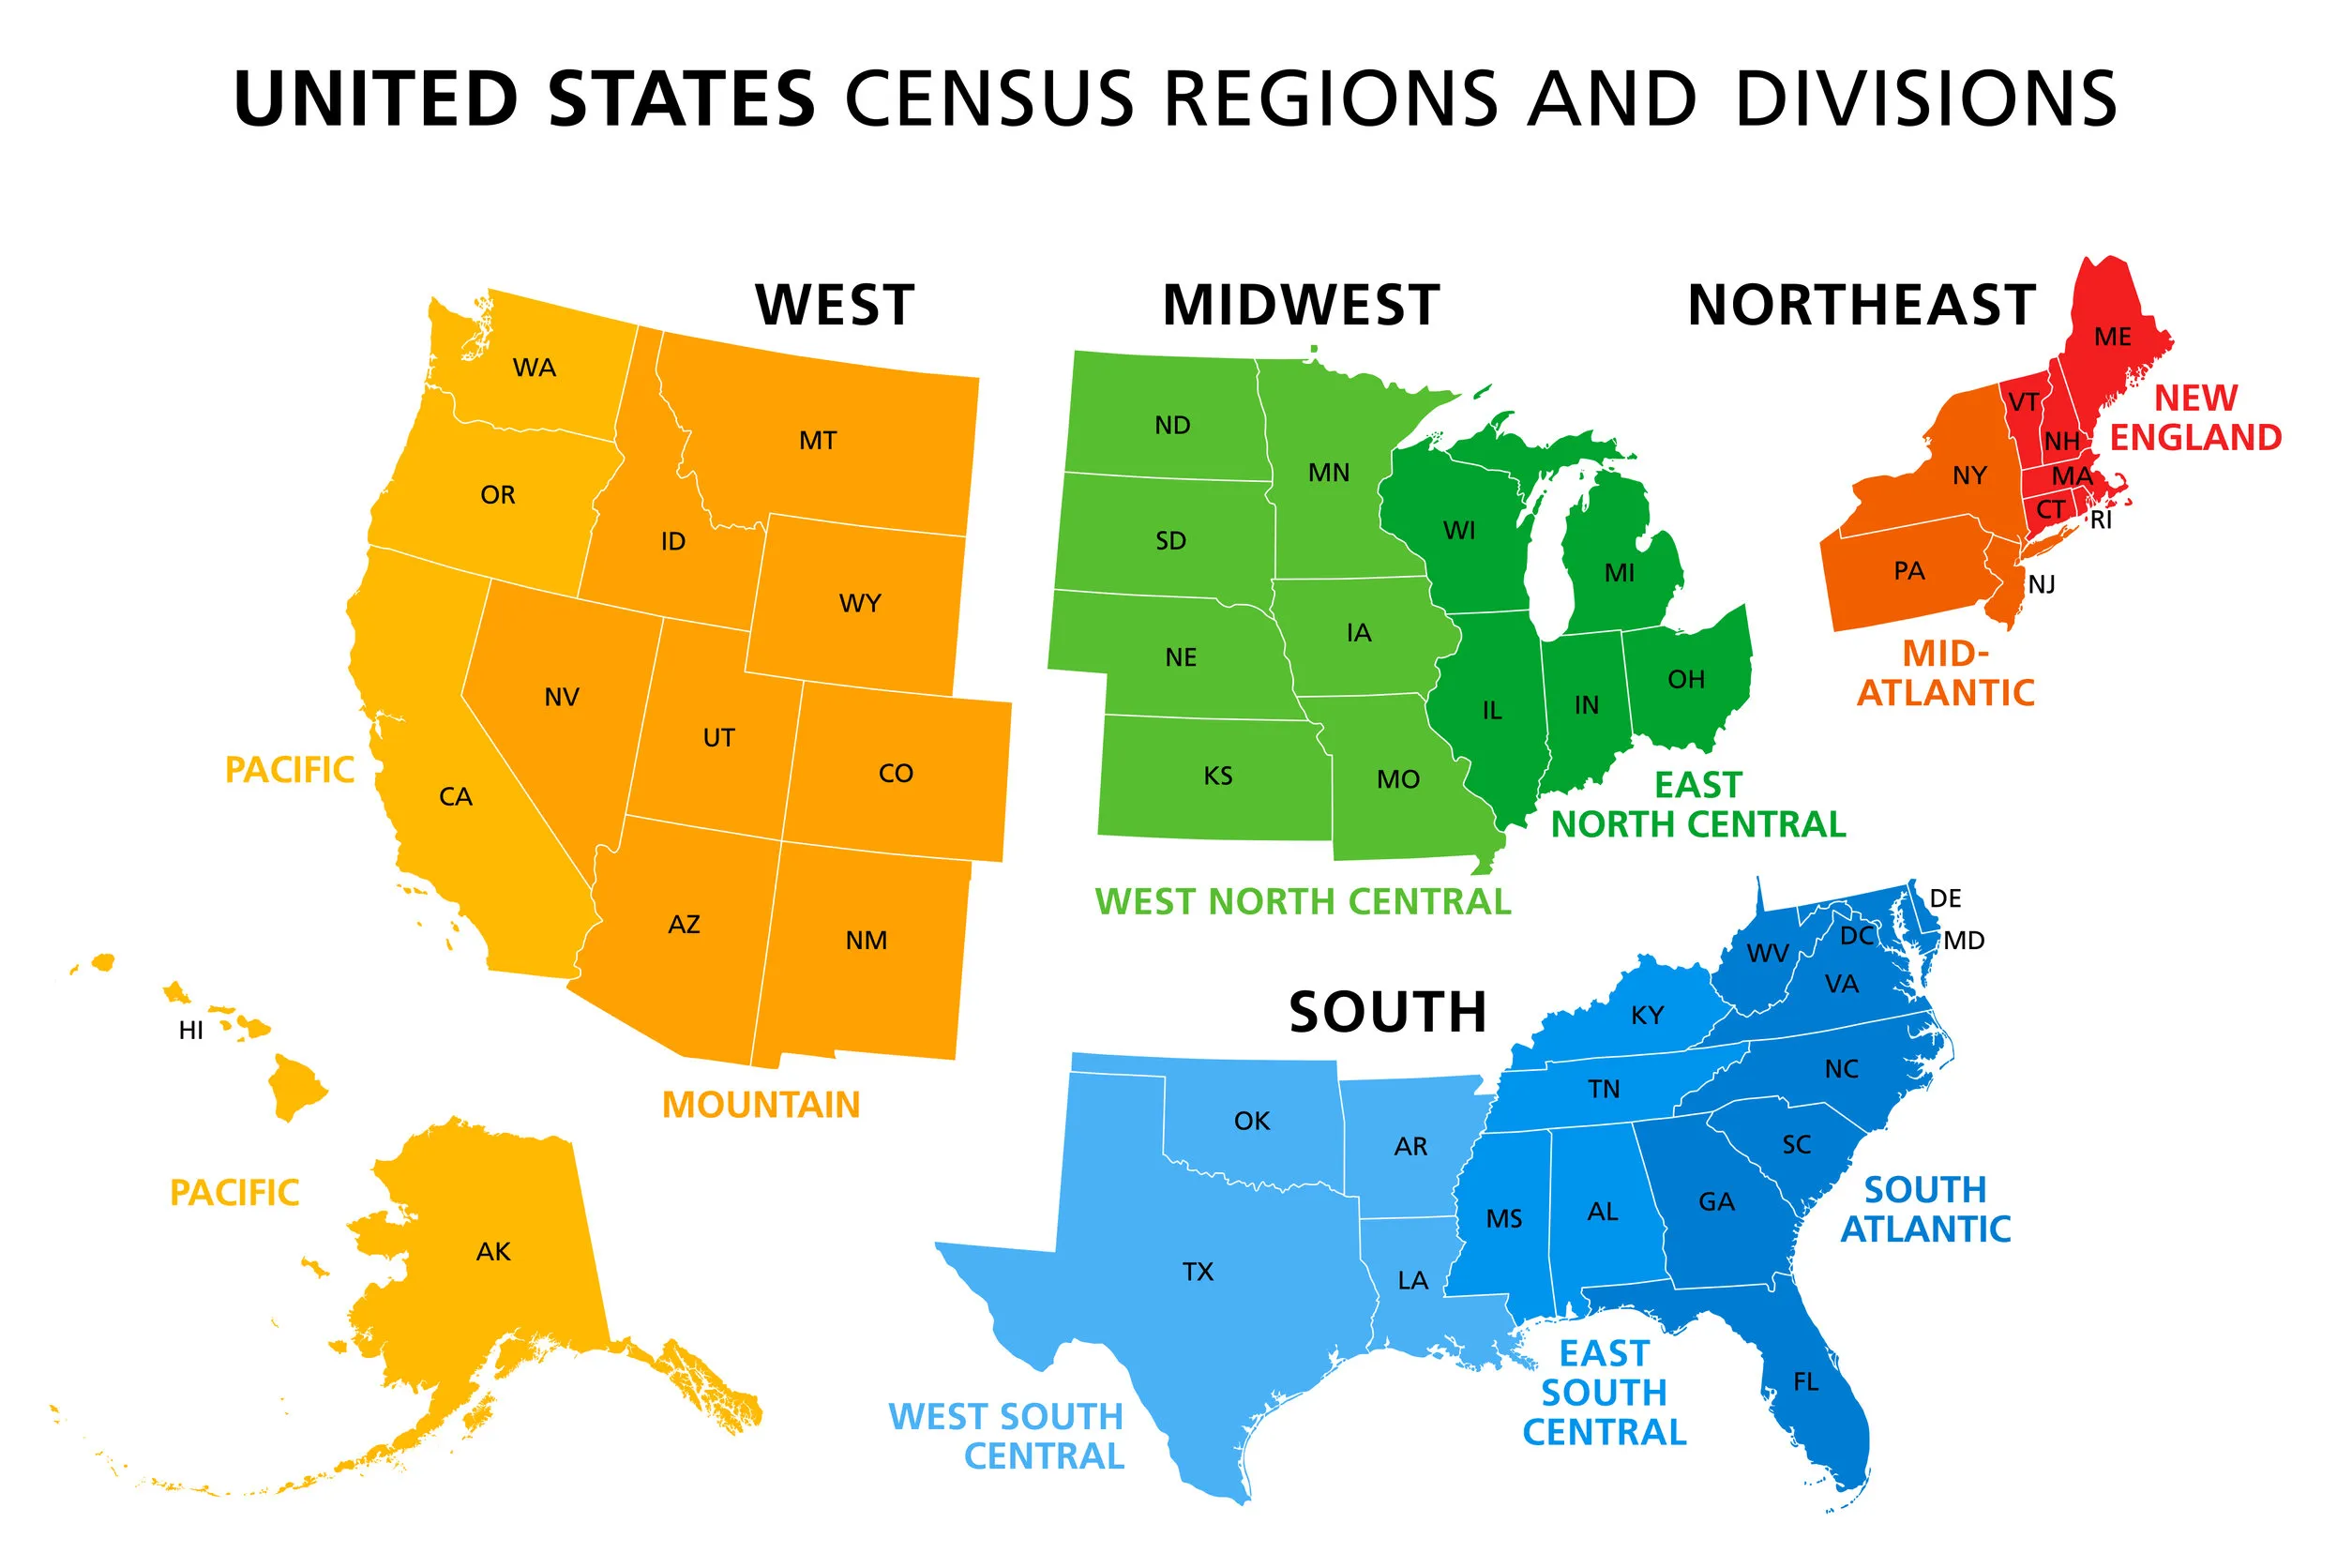
\includegraphics[scale=0.06]{us_regions.png}

\end{frame}

\begin{frame}{Linear regression with a categorical predictor}
What can we do? We can use \textcolor{blue}{dummy variables}\dots

\vspace{0.3cm}

\textcolor{blue}{Dummy variables}: The set of \textit{binary} variables created by re-writing (or re-coding) a multilevel categorical variable  

\vspace{0.3cm}

Example: Suppose we have a multilevel categorical variable for US region, with values West, Midwest, South, and Northeast

\vspace{0.3cm}

We create the new variables:
\begin{itemize}
	\item Midwest: \textit{Midwest} = 1 if \textit{region} = \textit{Midwest}, and 0 otherwise
	\item South: \textit{South} = 1 if \textit{region} = \textit{South}, and 0 otherwise
	\item Northeast: \textit{Northeast} = 1 if \textit{region} = \textit{Northeast}, and 0 otherwise
\end{itemize} \pause

\vspace{0.1cm}

\textcolor{blue}{Question:} We didn't make a dummy variable for West. Why not? \pause

\textcolor{blue}{Answer:} If all other dummy variables (Midwest, South, and Northeast) are 0, then the region must be West! In this case, West is referred to as a \textcolor{blue}{reference group}.
\end{frame} 

\begin{frame}{Linear regression with a categorical predictor}
Writing out our regression model for this example, we have
$$
E[\text{Outcome} \mid \text{Region}] = \beta_0 + \beta_1 \times \text{Midwest} + \beta_2 \times \text{South} + \beta_3 \times \text{Northeast}
$$

Note that we have more than just an intercept and slope coefficient here (making our way towards multiple linear regression!)

\vspace{0.3cm}

\textcolor{blue}{Question}: How do we interpret the coefficients $\beta_0$, $\beta_1$, $\beta_2$, $\beta_3$? \pause

\vspace{0.3cm}

$\beta_0$: average outcome among those in the Western region

$$
E[\text{Outcome} \mid \text{Region = West}] = \beta_0 + \beta_1 \times 0 + \beta_2 \times 0 + \beta_3 \times 0
$$


\end{frame}

\begin{frame}{Linear regression with a categorical predictor}
Writing out our regression model for this example, we have
$$
E[\text{Outcome} \mid \text{Region}] = \beta_0 + \beta_1 \times \text{Midwest} + \beta_2 \times \text{South} + \beta_3 \times \text{Northeast}
$$

Note that we have more than just an intercept and slope coefficient here (making our way towards multiple linear regression!)

\vspace{0.3cm}

\textcolor{blue}{Question}: How do we interpret the coefficients $\beta_0$, $\beta_1$, $\beta_2$, $\beta_3$?

\vspace{0.3cm}

$\beta_1$: difference in average outcome between groups in the Western region and Midwest region

\begin{align*}
E[&\text{Outcome} \mid  \text{Region = Midwest}] - E[\text{Outcome} \mid \text{Region = West}] \\
& = [\beta_0 + \beta_1 \times 1 + \beta_2 \times 0 + \beta_3 \times 0] - [\beta_0 + \beta_1 \times 0 + \beta_2 \times 0 + \beta_3 \times 0] \\
& = \beta_0 + \beta_1 - \beta_0 \\
& = \beta_1
\end{align*}


\end{frame}

\begin{frame}{Linear regression with a categorical predictor}
Writing out our regression model for this example, we have
$$
E[\text{Outcome} \mid \text{Region}] = \beta_0 + \beta_1 \times \text{Midwest} + \beta_2 \times \text{South} + \beta_3 \times \text{Northeast}
$$

Note that we have more than just an intercept and slope coefficient here (making our way towards multiple linear regression!)

\vspace{0.3cm}

\textcolor{blue}{Question}: How do we interpret the coefficients $\beta_0$, $\beta_1$, $\beta_2$, $\beta_3$?

\vspace{0.3cm}

$\beta_2$: difference in average outcome between groups in the Western region and Southern region

\begin{align*}
E[&\text{Outcome} \mid  \text{Region = South}] - E[\text{Outcome} \mid \text{Region = West}] \\
& = [\beta_0 + \beta_1 \times 0 + \beta_2 \times 1 + \beta_3 \times 0] - [\beta_0 + \beta_1 \times 0 + \beta_2 \times 0 + \beta_3 \times 0] \\
& = \beta_0 + \beta_2 - \beta_0 \\
& = \beta_2
\end{align*}


\end{frame}

\begin{frame}{Linear regression with a categorical predictor}
Writing out our regression model for this example, we have
$$
E[\text{Outcome} \mid \text{Region}] = \beta_0 + \beta_1 \times \text{Midwest} + \beta_2 \times \text{South} + \beta_3 \times \text{Northeast}
$$

Note that we have more than just an intercept and slope coefficient here (making our way towards multiple linear regression!)

\vspace{0.3cm}

\textcolor{blue}{Question}: How do we interpret the coefficients $\beta_0$, $\beta_1$, $\beta_2$, $\beta_3$?

\vspace{0.3cm}

$\beta_3$: difference in average outcome between groups in the Western region and Northeastern region

\begin{align*}
E[&\text{Outcome} \mid  \text{Region = Northeast}] - E[\text{Outcome} \mid \text{Region = West}] \\
& = [\beta_0 + \beta_1 \times 0 + \beta_2 \times 0 + \beta_3 \times 1] - [\beta_0 + \beta_1 \times 0 + \beta_2 \times 0 + \beta_3 \times 0] \\
& = \beta_0 + \beta_3 - \beta_0 \\
& = \beta_3
\end{align*}

\end{frame}

\begin{frame}{Linear regression with a categorical predictor: summary}
Our example:
$$
E[\text{Outcome} \mid  \text{Region = Northeast}] - E[\text{Outcome} \mid \text{Region = West}] 
$$

\begin{itemize}
	\item If we have $k$ categories, we create $k - 1$ \textcolor{blue}{dummy variables}, with the $k$th category being the \textcolor{blue}{reference group} captured in the intercept
	\item \texttt{R} automatically creates these dummy variables for you for multilevel categorical variables, as you'll see on your homework
\end{itemize}

\vspace{0.3cm}

Hypothesis testing: If we want to test whether our outcome is associated with a multilevel categorical variable, we need to test if \textit{all} coefficients for the dummy variables (in this example, $\beta_1, \beta_2, \beta_3$) are equal to zero.

\end{frame}

\begin{frame}{Linear regression with a categorical predictor: Example in \texttt{R}}
Suppose we're interested in whether birthweight is associated with race, in our births dataset. We can fit a linear regression model as before with simple linear regression, and look at the output\dots

\vspace{0.3cm}

\centering

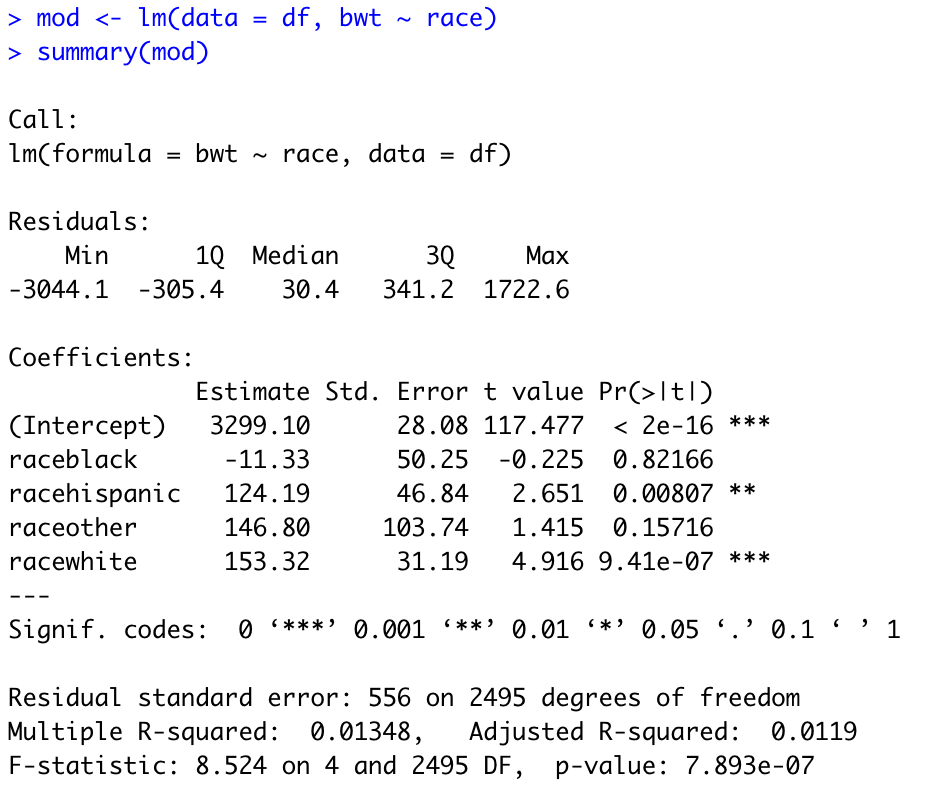
\includegraphics[scale=0.4]{multilevel_cat_lm.png}

\end{frame}

\begin{frame}{Linear regression with a categorical predictor: Example in \texttt{R}}

\begin{figure}
	\centering 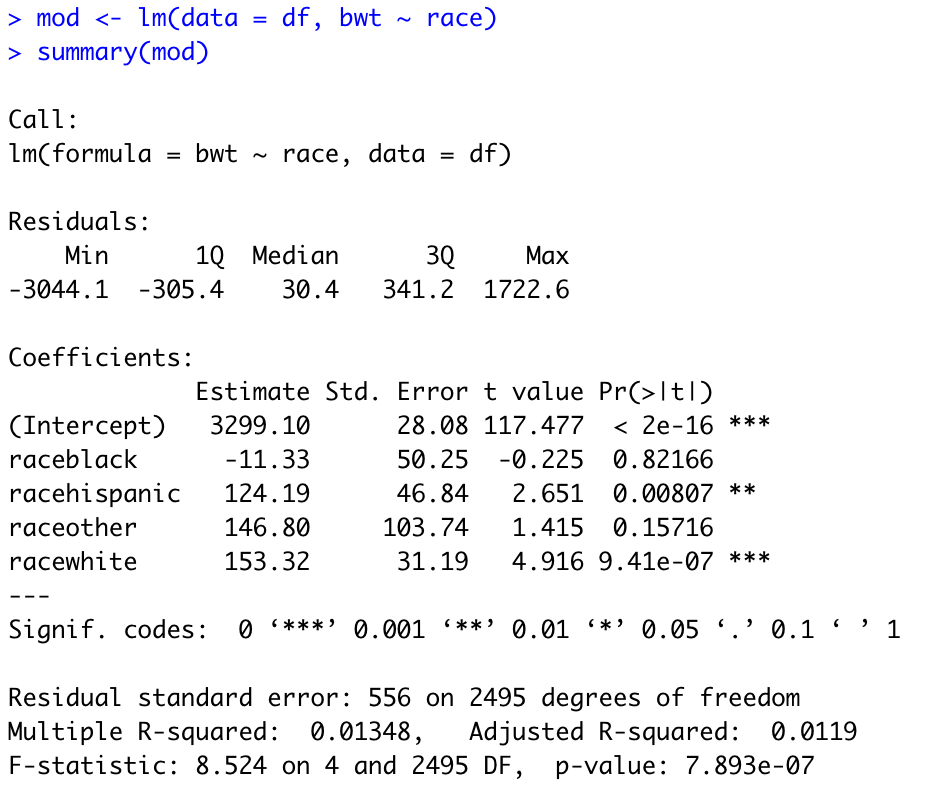
\includegraphics[scale=0.3]{multilevel_cat_lm.png}
\end{figure}

\vspace{0.1cm}

A couple things to notice:


\end{frame}

\begin{frame}{Linear regression with a categorical predictor: Example in \texttt{R}}

\begin{figure}
	\centering 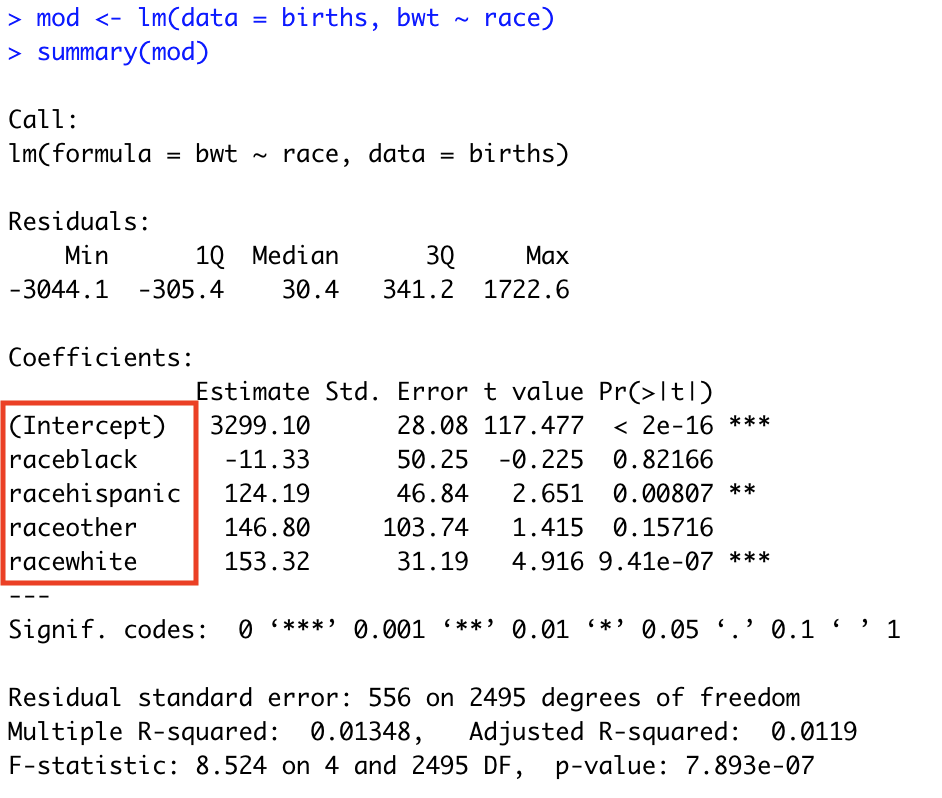
\includegraphics[scale=0.3]{multilevel_cat_lm2.png}
\end{figure}

\vspace{0.1cm}

A couple things to notice:
\begin{itemize}
	\item \texttt{R} has created dummy variables for us! The reference group by default will be the first category alphabetically (in this case, ``asian").
\end{itemize}

\end{frame}

\begin{frame}{Linear regression with a categorical predictor: Example in \texttt{R}}

\begin{figure}
	\centering 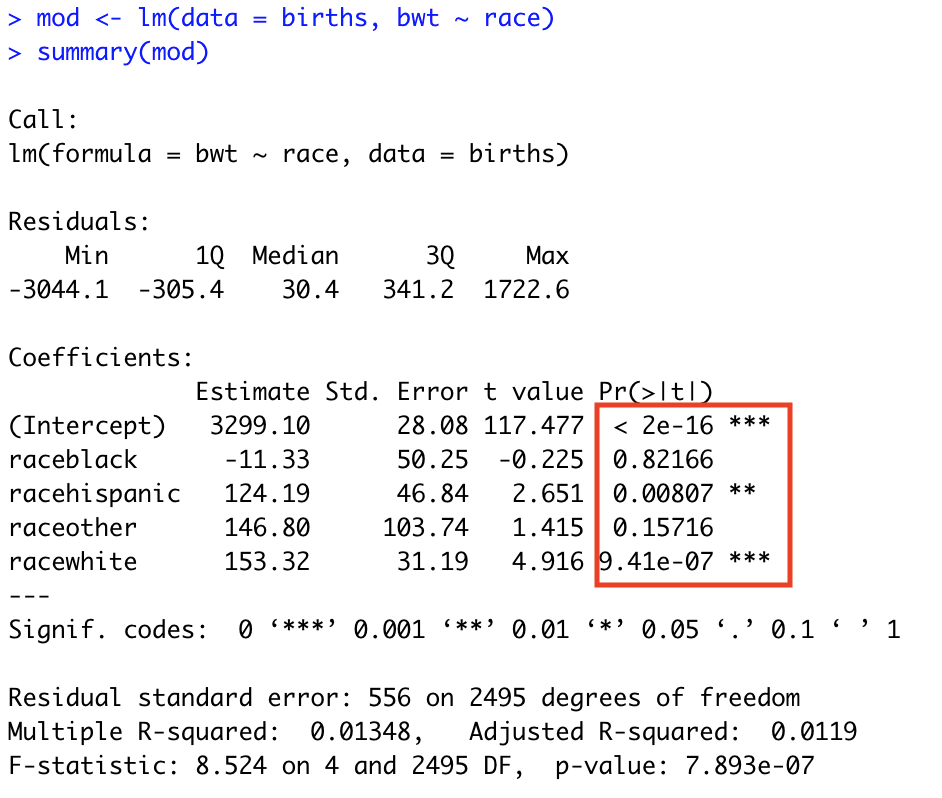
\includegraphics[scale=0.3]{multilevel_cat_lm3.png}
\end{figure}

\vspace{0.1cm}

A couple things to notice:
\begin{itemize}
	\item We have multiple p-values! But which p-value is the one associated with our hypothesis test? Let's write it down\dots
\end{itemize}

\end{frame}

\begin{frame}{Linear regression with a categorical predictor: Example in \texttt{R}}
We're interested in whether birthweight is associated with race, in our births dataset. Our regression model has the form:
$$
E[\text{bwt} \mid \text{race}] = \beta_0 + \beta_1 \times \text{black} + \beta_2 \times \text{hispanic} + \beta_3 \times \text{other} + \beta_4 \times \text{white}
$$ \pause

Our null hypthesis (in words) is that there is no association between race and birthweight. This would mean that \textcolor{blue}{all dummy variables for race} are \textit{simultaneously} equal to zero. \pause In math:

\vspace{0.3cm}

\begin{itemize}
	\item $H_0$: $\beta_1 = \beta_2 = \beta_3 = 0$
	\item $H_1$: \textit{at least one} of $\beta_1, \beta_2, \beta_3$ is not equal to $0$
\end{itemize} \pause

\vspace{0.3cm}

How do we do this in \texttt{R}?

\end{frame}

\begin{frame}{Linear regression with a categorical predictor: Example in \texttt{R}}
In \texttt{R}, we create two linear regression models: one with the race variable and an intercept, and one with only an intercept. We then use the \texttt{anova} function to test whether the race variable as a whole is significantly associated with birthweight.

\vspace{0.3cm}

\texttt{mod1 <- lm(data = df, bwt} $\sim$ \texttt{1) \\
	mod2 <- lm(data = df, bwt} $\sim$ \texttt{race) \\
	anova(mod1, mod2)} \pause

\vspace{0.3cm}

Details:
\begin{itemize}
	\item \texttt{mod1} is the model with only an intercept (specified with the $1$ on the right hand side of the tilde)
	\item Inside of the \texttt{anova} function, we put the ``smaller" model first (in this case, the model without the race covariate)
\end{itemize}
\end{frame}

\begin{frame}{Linear regression with a categorical predictor: Example in \texttt{R}}

Our output from the \texttt{anova} function:

\vspace{0.3cm}

\begin{figure}
	\centering 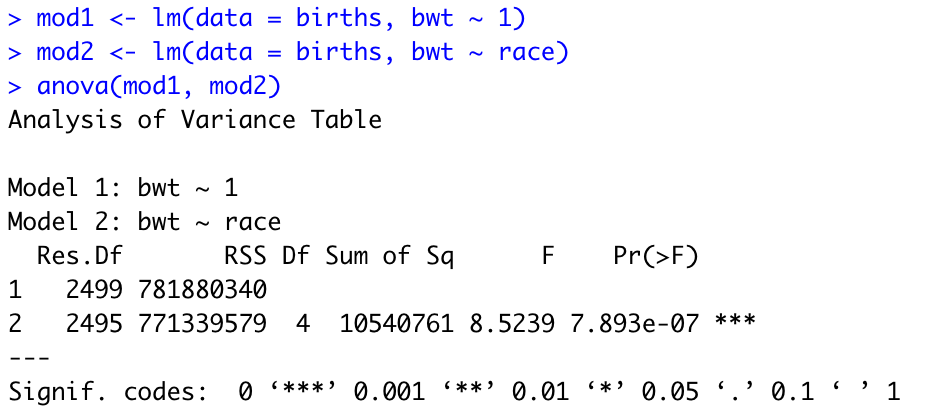
\includegraphics[scale=0.4]{anova_race.png}
\end{figure}

\end{frame}

\begin{frame}{Linear regression with a categorical predictor: Example in \texttt{R}}
Our output from the \texttt{anova} function:

\vspace{0.3cm}

\begin{figure}
	\centering 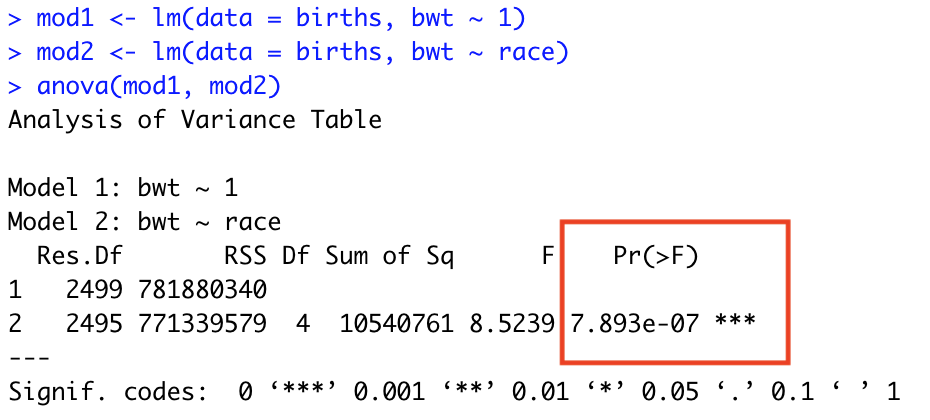
\includegraphics[scale=0.4]{anova_race2.png}
\end{figure}

\vspace{0.3cm}

\textit{This} is the p-value for our hypothesis test. \textit{Not} the individual p-values from our linear regression output. \pause

\vspace{0.3cm}



\includegraphics[scale=0.01]{chilipepper.png} \tiny You might notice that the p-value here corresponds to an F statistic, as opposed to a $t$ statistic as with hypothesis tests for single coefficients (e.g., $\beta_1 = 0$ vs. $\beta_1 \neq 0$). The key here is that F tests allow us to test for multiple coefficients being equal to $0$ at once. If you're interested in mathematical details, please ask us!

\end{frame}

\begin{frame}{Linear regression with a categorical predictor: Example in \texttt{R}}
Key Takeaway(s):
\vspace{0.3cm}

\begin{itemize}
	\item The individual p-values for separate categories of a multilevel categorical variable \textit{do not} correspond to the hypothesis test for whether the variable is associatied with the outcome
	\item We use the \texttt{anova} function in \texttt{R} to get p-values that correspond to hypothesis tests where the null hypothesis involves setting \textit{more than one} coefficient equal to zero
\end{itemize} \pause

\vspace{0.3cm}

What does this example have to do with multiple linear regression? 

\vspace{0.3cm}

Multiple linear regression involves having \textit{multiple} predictors in your model. Multilevel categorical variables are a preview of multiple linear regression, as they can be framed as multiple dummy variables! \pause

\vspace{0.2cm}

\tiny *note that the polynomial transformation also involved multiple predictors in our model, so you've now had two previews of multiple linear regression

\end{frame}

\subsection{Graphical examples}

\begin{frame}{Multiple linear regression: Motivation}
So far, we have considered the relationship between the outcome $Y$ and a single covariate/predictor $X$. Some terminology we'll use:

\vspace{0.3cm}

\textcolor{blue}{Predictor of interest}: the covariate whose relationship to the outcome corresponds to our primary scientific/statistical question \pause

\vspace{0.3cm}

In everything we've done so far $X$ has been our predictor of interest, but it also been our \textit{only} predictor. However, there may be other variables that \textit{influence} the association between our predictor of interest and the outcome, by:

\vspace{0.3cm}

\begin{itemize}
	\item \textcolor{blue}{Confounding} the association
	\item \textcolor{blue}{Modifying} the association
	\item Providing information that \textcolor{blue}{reduces the variability} of our estimates
\end{itemize}

\end{frame}

\begin{frame}{Multiple linear regression: Motivation}
(1) Suppose we collect information on the variables $X_1$ and $Y$ for 50 individuals (plotted below). What is your best guess at the linear relationship between $X_1$ and $Y$ (i.e. how would you draw the simple linear regression line on this graph)?

\vspace{0.3cm}

\centering 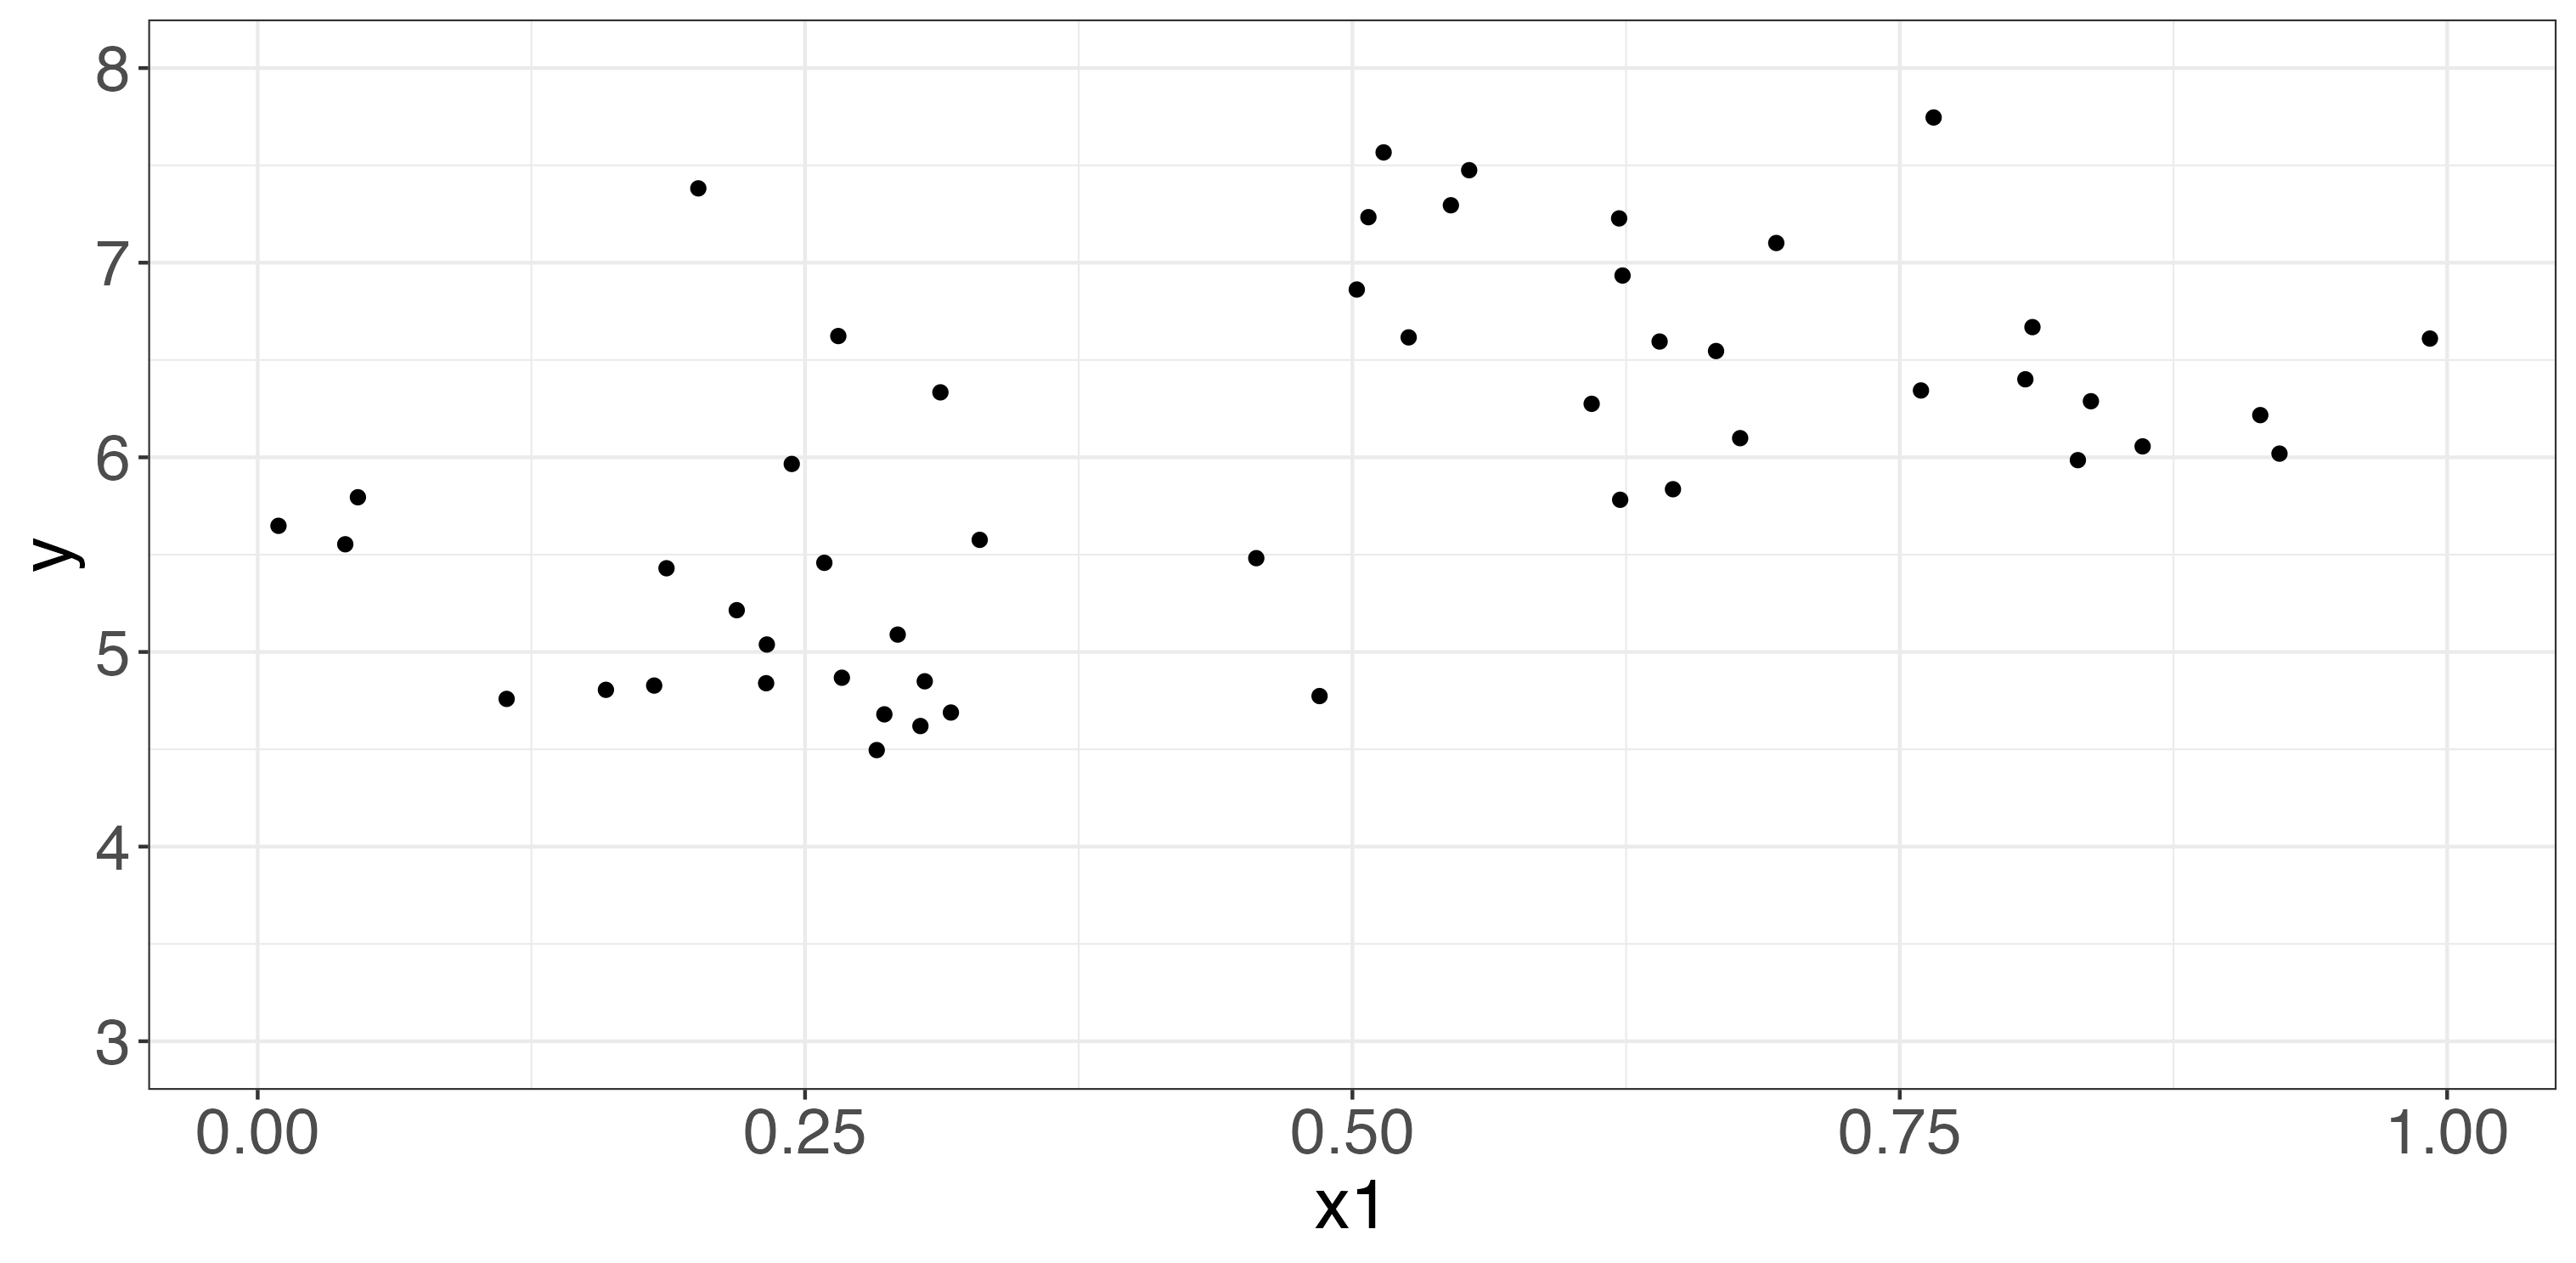
\includegraphics[scale=0.3]{multreg1.png}
\end{frame}

\begin{frame}{Multiple linear regression: Motivation}
(1) Suppose we collect information on the variables $X_1$ and $Y$ for 50 individuals (plotted below). What is your best guess at the linear relationship between $X_1$ and $Y$ (i.e. how would you draw the simple linear regression line on this graph)?

\vspace{0.3cm}

\centering 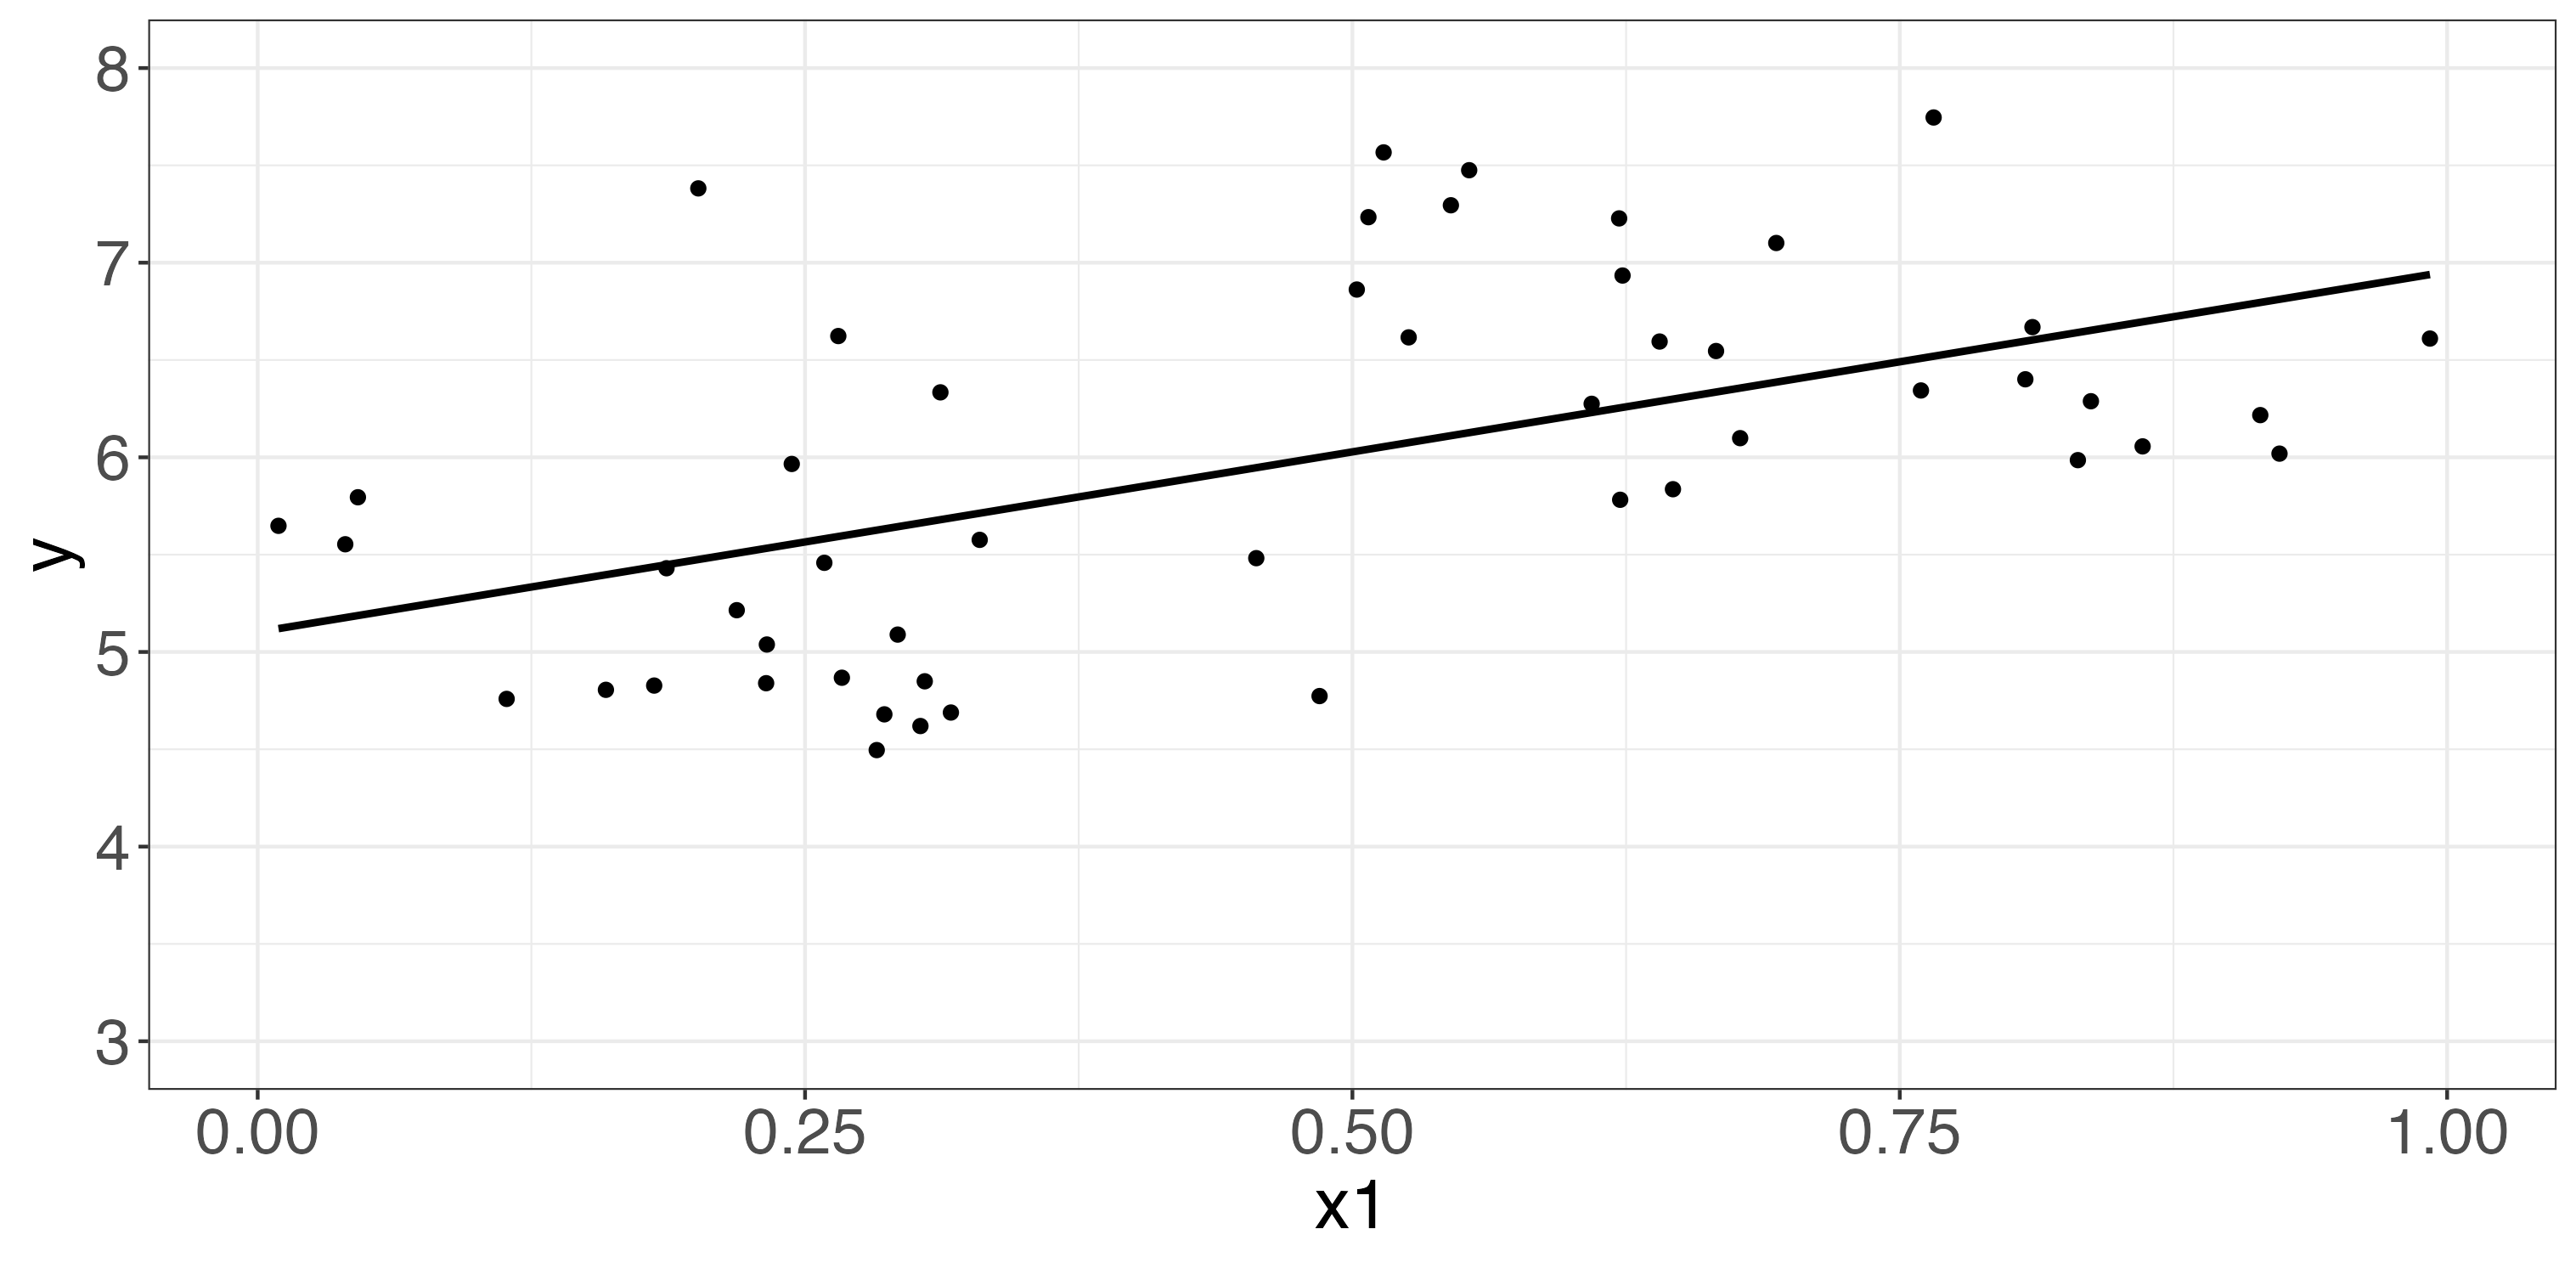
\includegraphics[scale=0.3]{multreg2.png}
\end{frame}

\begin{frame}{Multiple linear regression: Motivation}
(2) Suppose we also collected information on the binary variable $X_2$ for each individual. What is your best guess at the linear relationship between $X_1$ and $Y$, \textit{for each group} defined by the variable $X_2$? 

\vspace{0.3cm}

\centering 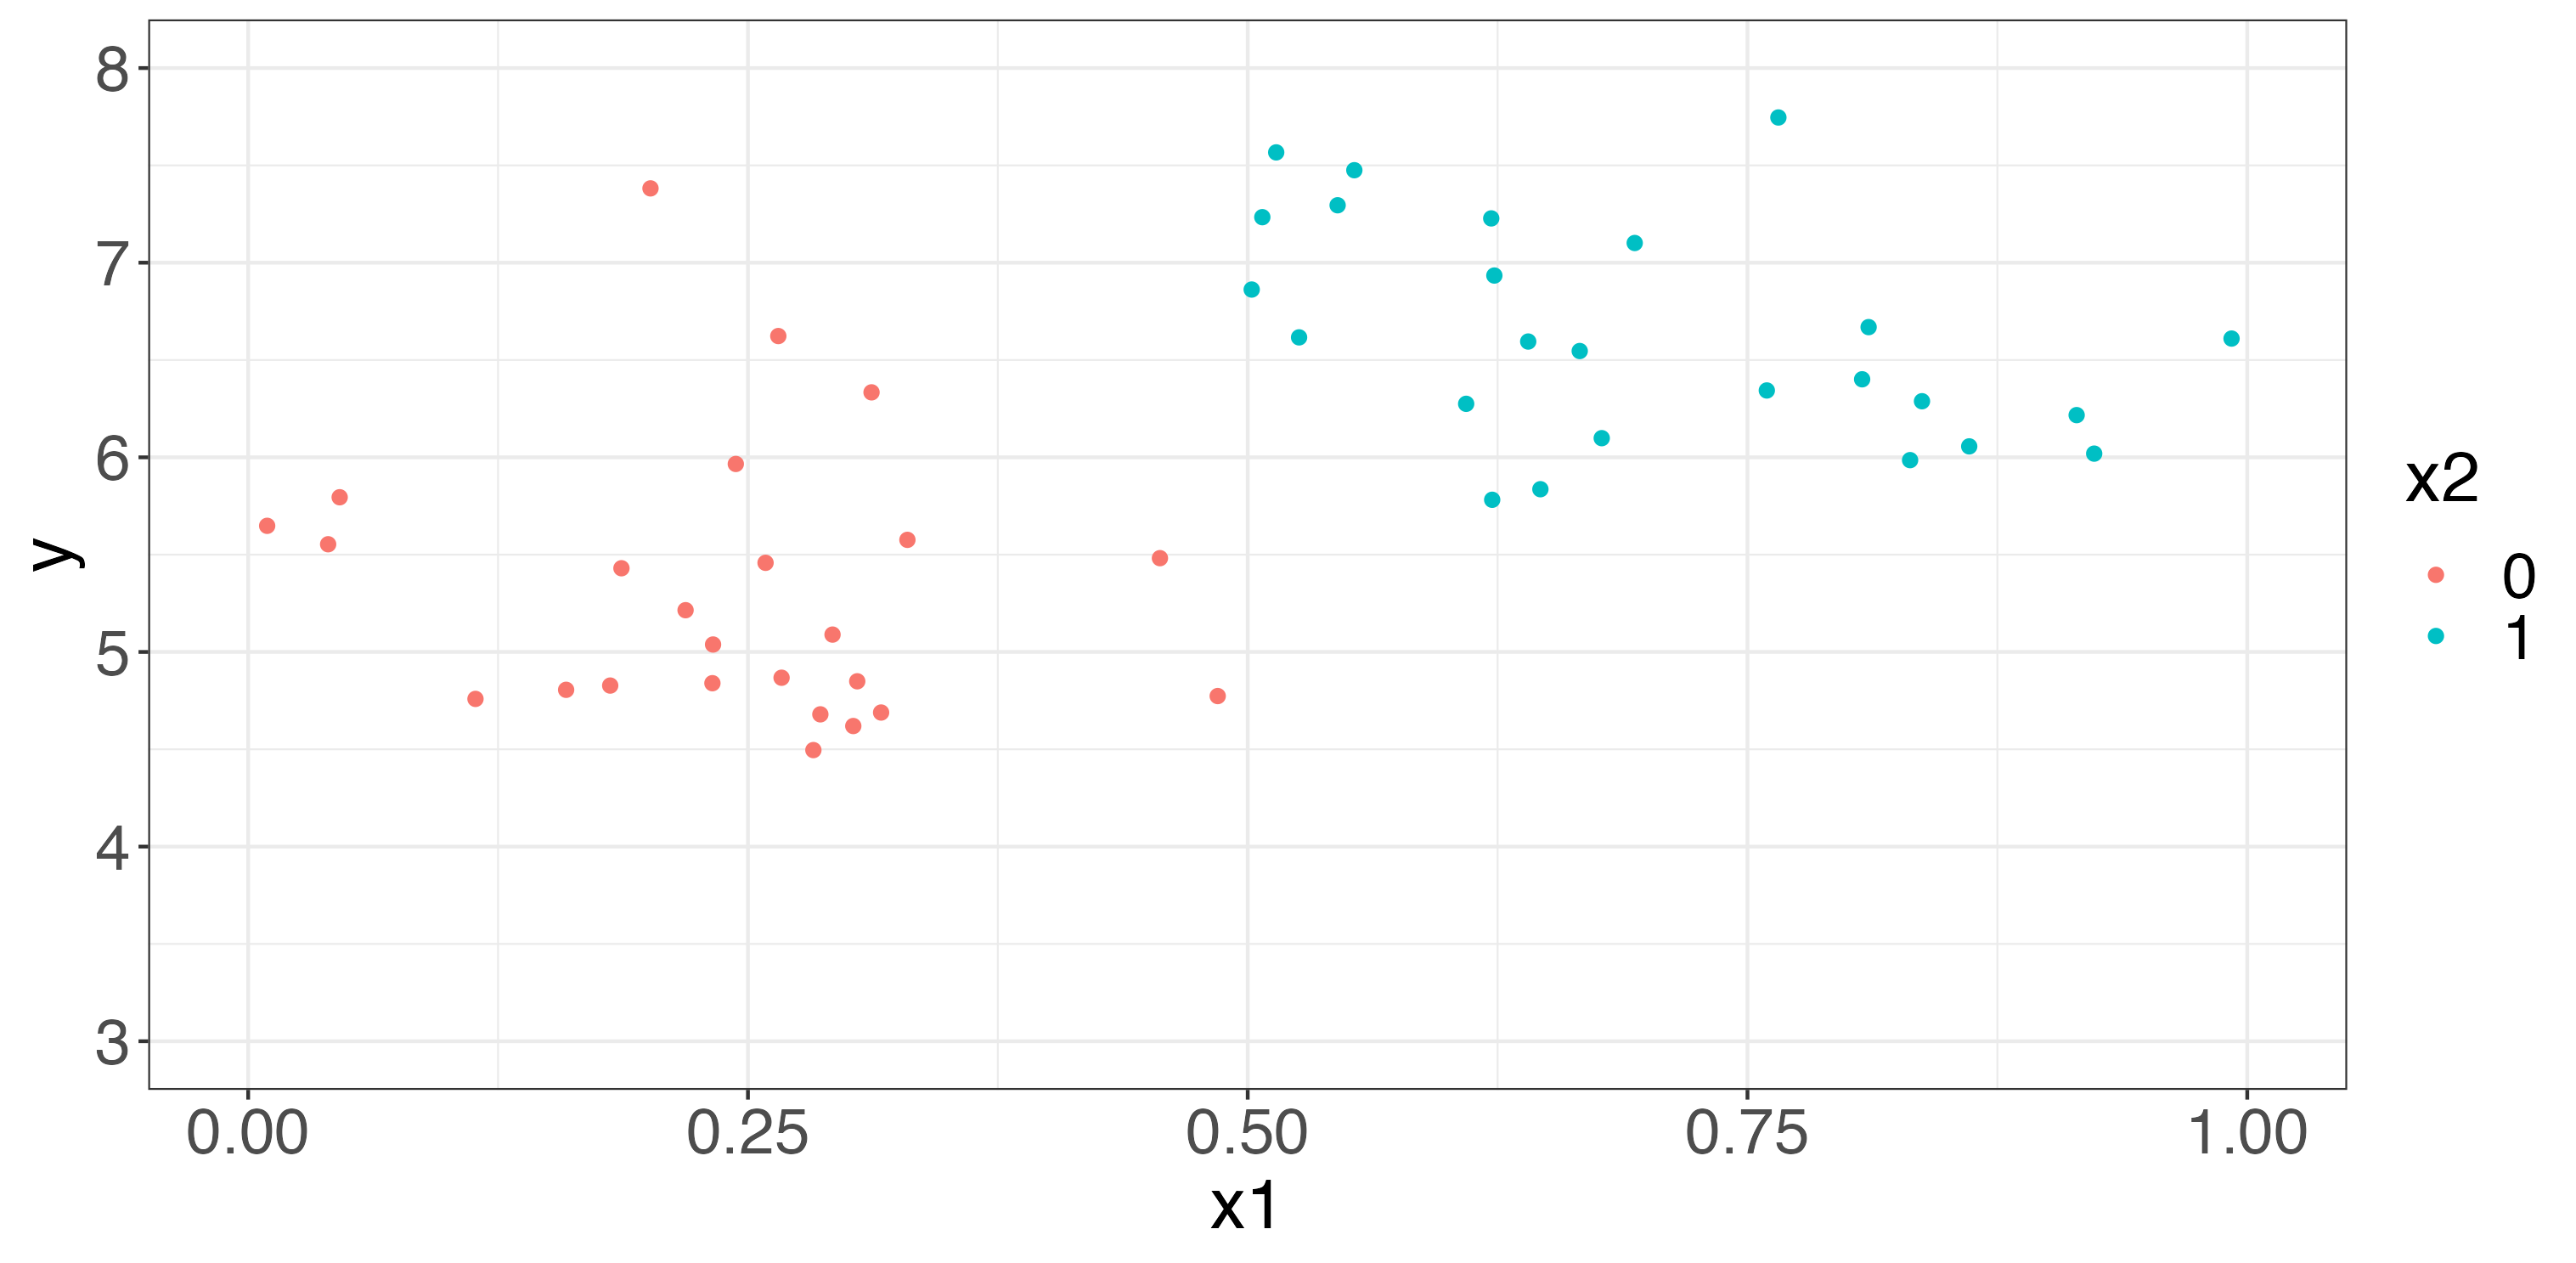
\includegraphics[scale=0.3]{multreg3.png}

\end{frame}

\begin{frame}{Multiple linear regression: Motivation}
(2) Suppose we also collected information on the binary variable $X_2$ for each individual. What is your best guess at the linear relationship between $X_1$ and $Y$, \textit{for each group} defined by the variable $X_2$? 

\vspace{0.3cm}

\centering 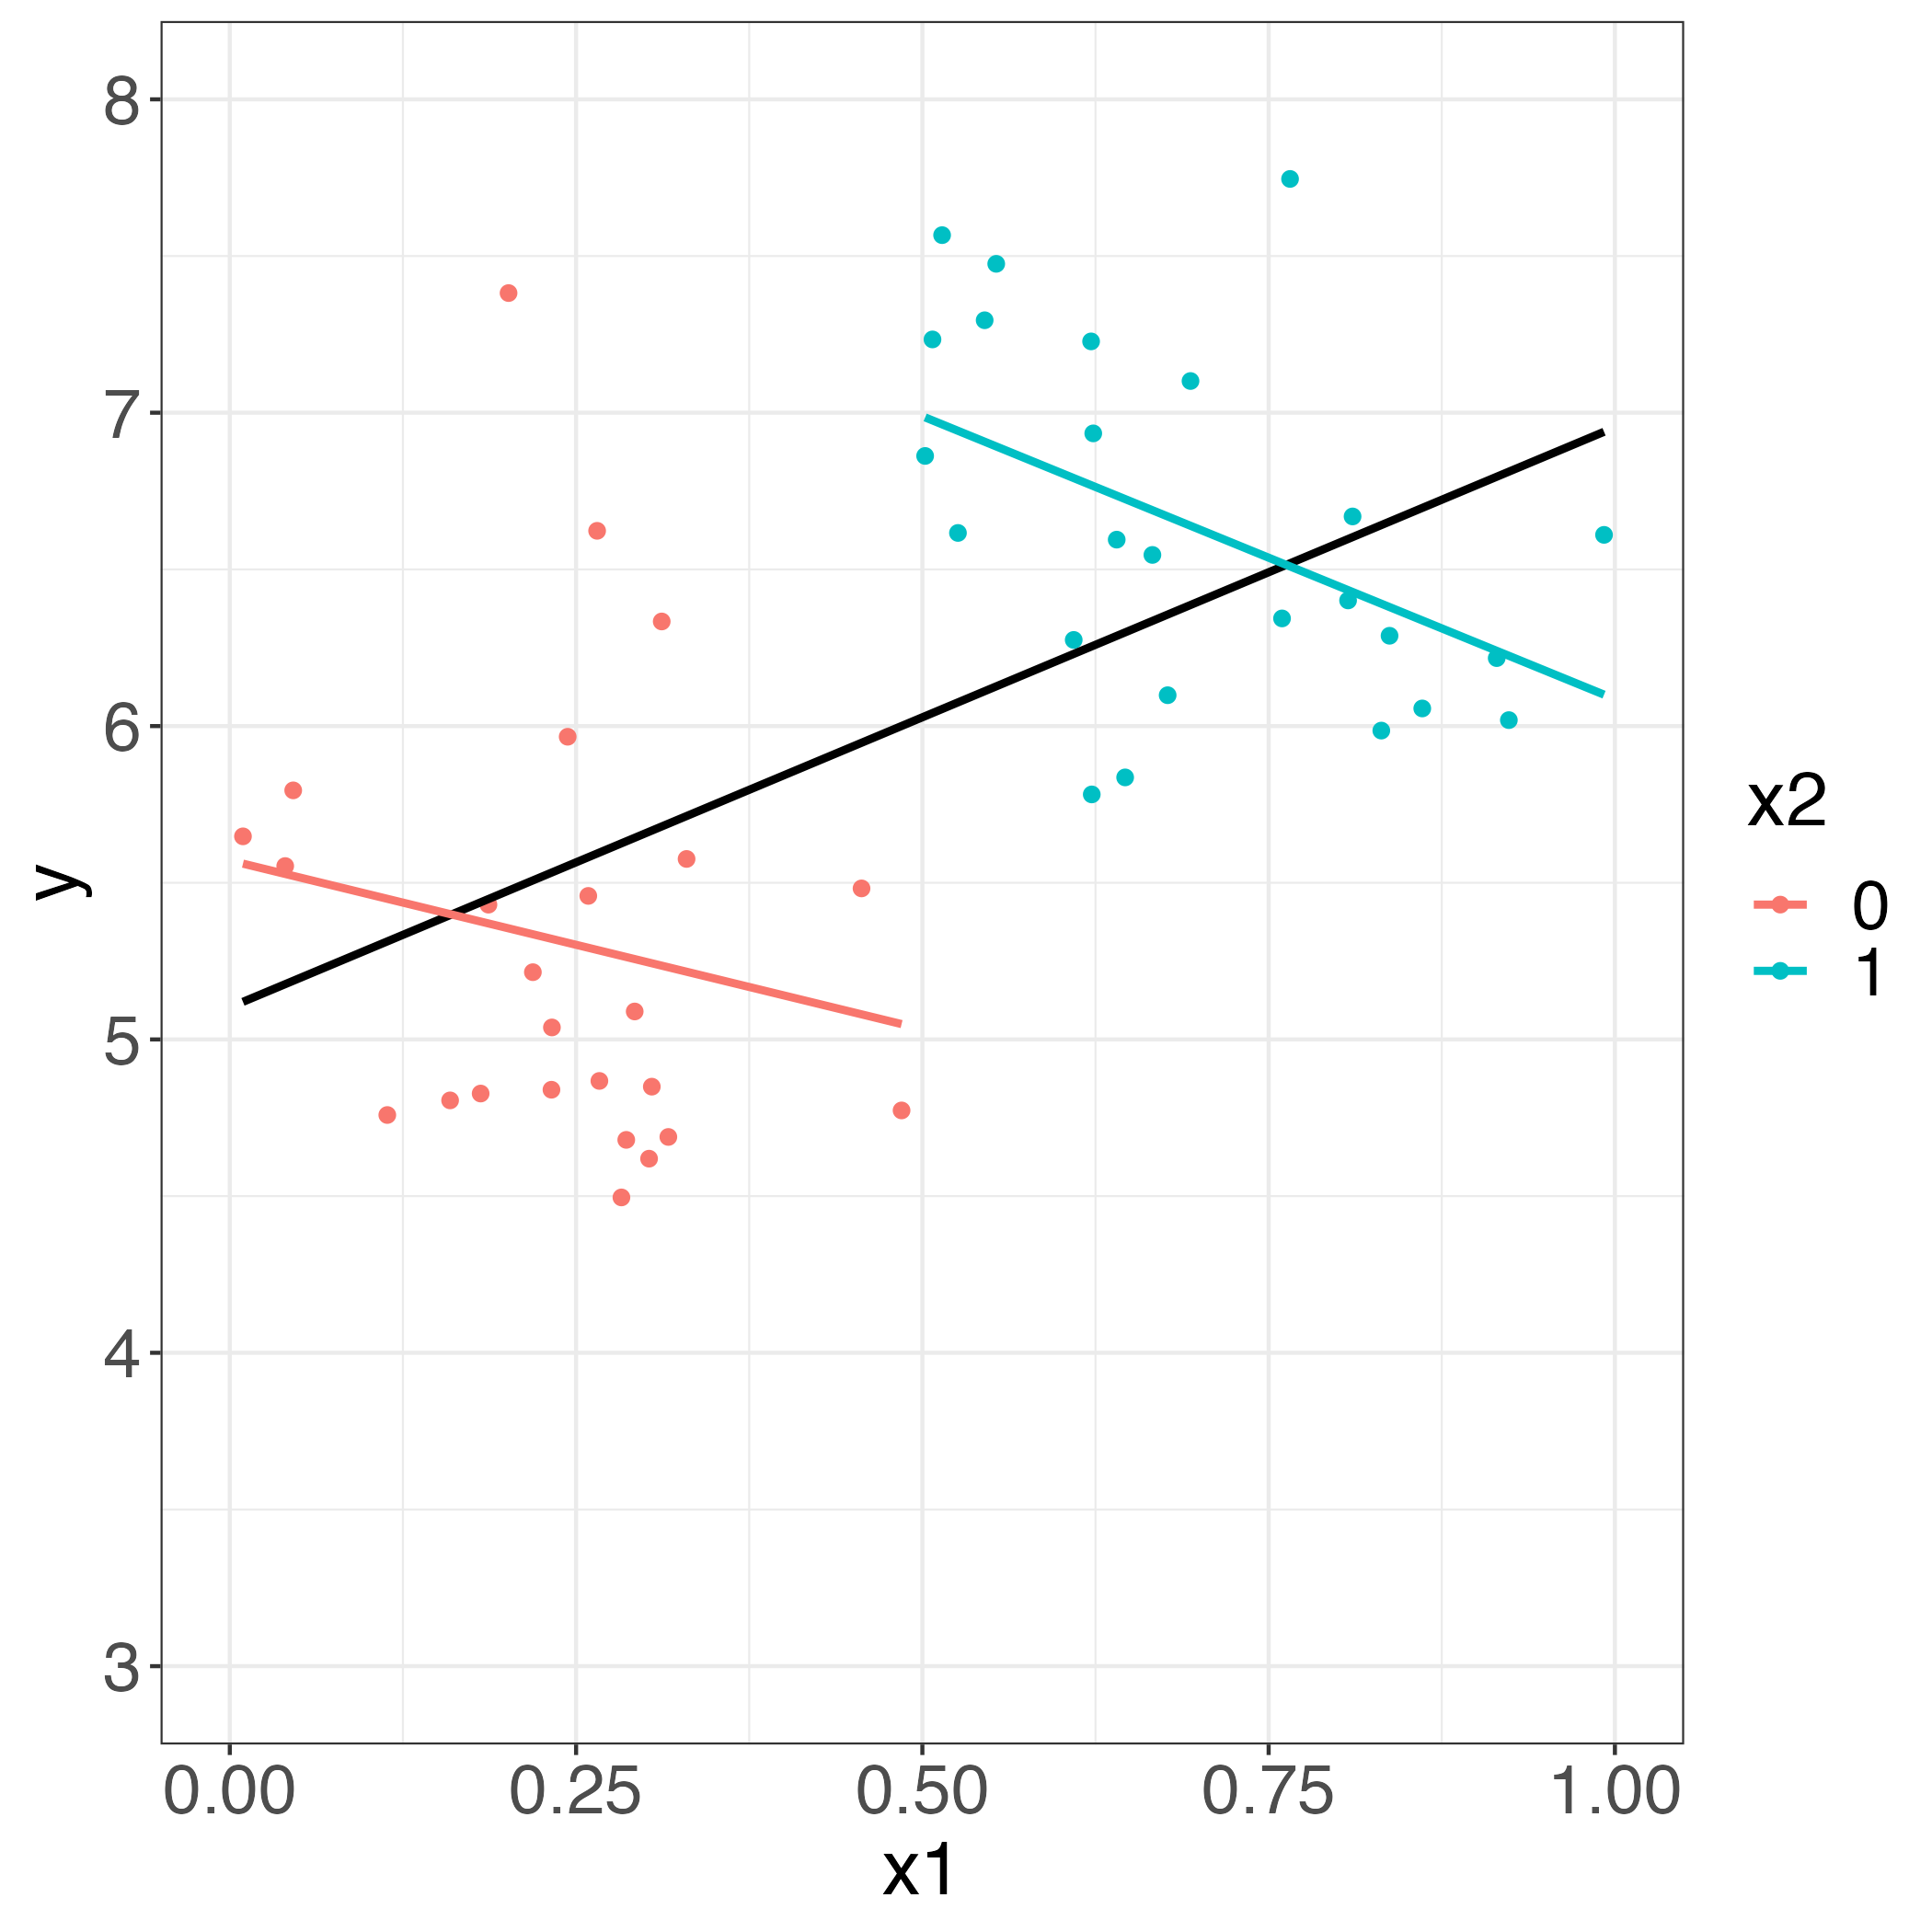
\includegraphics[scale=0.3]{multreg4.png}

\end{frame}

\begin{frame}{Multiple linear regression: Motivation}
\begin{figure}
	\centering 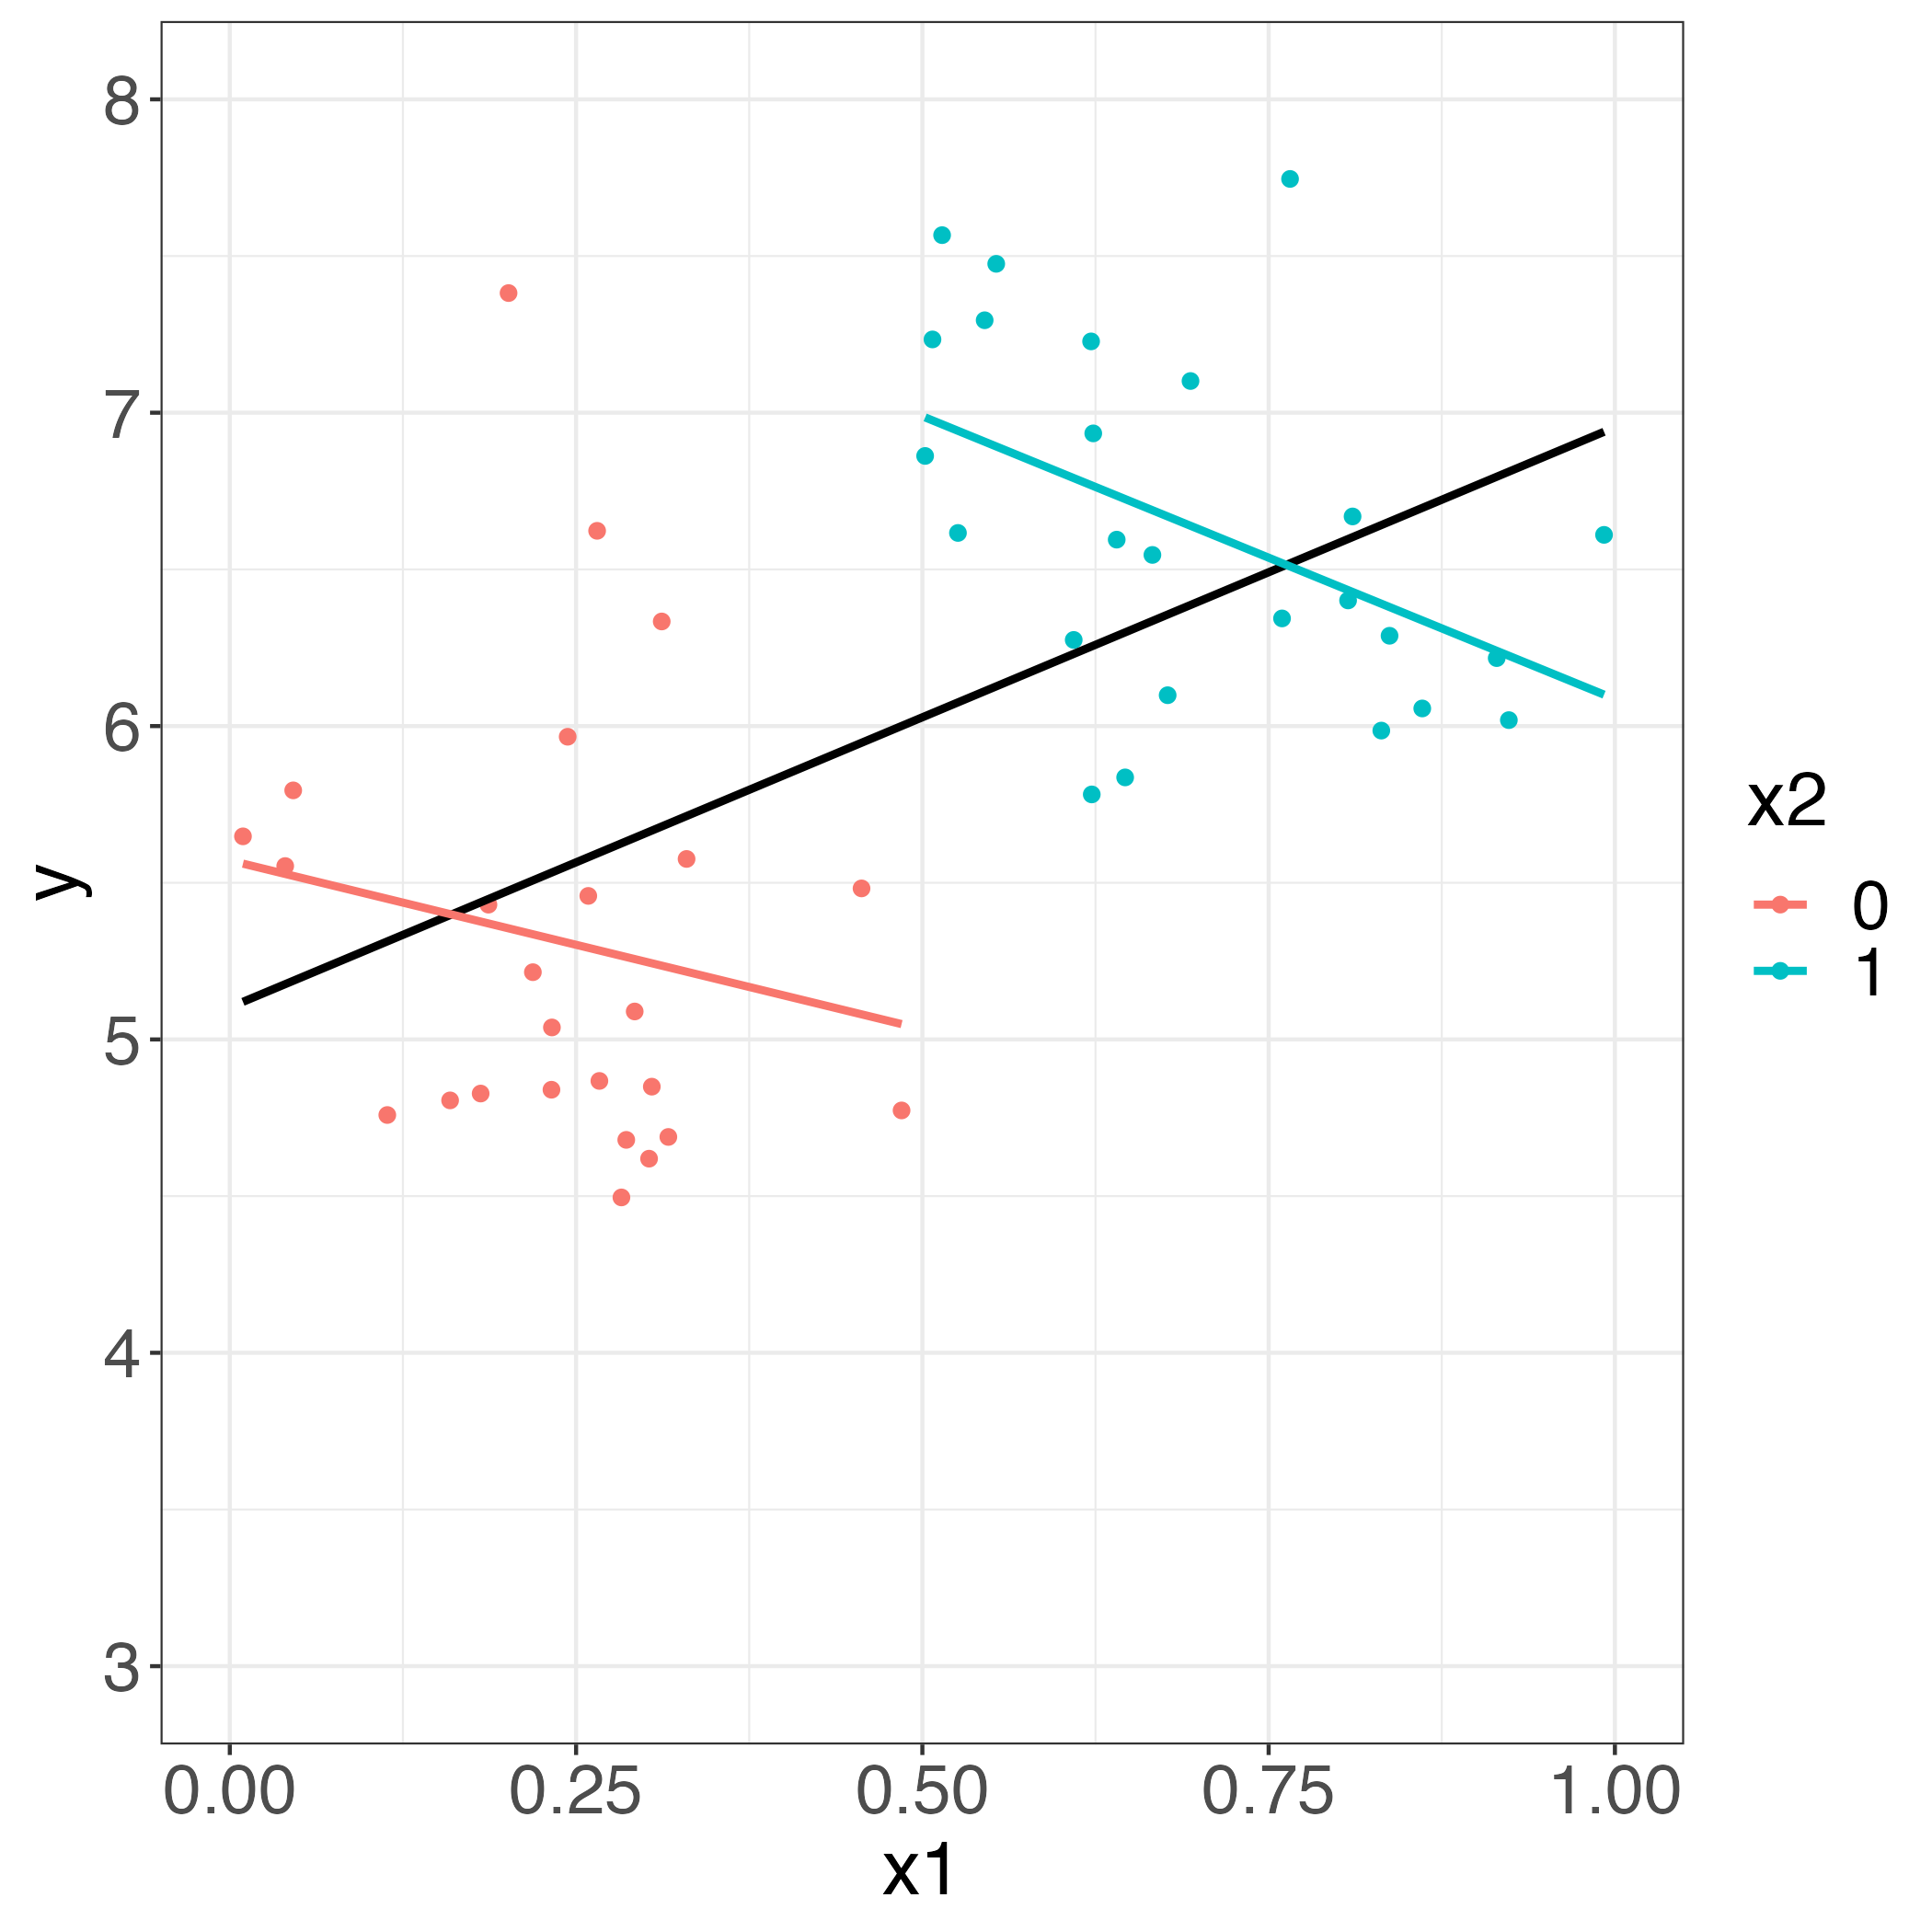
\includegraphics[scale=0.2]{multreg4.png}
\end{figure}

\vspace{0.1cm}

A couple things to note:

\begin{itemize}
	\item The best fitting line for the relationship between $X_1$ and $Y$ is different when we ignore $X_2$ vs. the best fitting lines for the relationship between $X_1$ and $Y$ for each group defined by $X_2$
	\item The lines we drew were in response to \textit{different} questions:
	\begin{enumerate}
		\item What is your best guess at the linear relationship between $X_1$ and $Y$?
		\item What is your best guess at the linear relationship between $X_1$ and $Y$, \textit{for each group} defined by the variable $X_2$? 
	\end{enumerate}
\end{itemize}

\end{frame}

\begin{frame}{Multiple linear regression: Motivation}
\begin{itemize}
	\item The best fitting line for the relationship between $X_1$ and $Y$ is different when we ignore $X_2$ vs. the best fitting lines for the relationship between $X_1$ and $Y$ for each group defined by $X_2$
	\item The lines we drew were in response to \textit{different} questions:
	\begin{enumerate}
		\item What is your best guess at the linear relationship between $X_1$ and $Y$?
		\item What is your best guess at the linear relationship between $X_1$ and $Y$, \textit{for each group} defined by the variable $X_2$? 
	\end{enumerate}
\end{itemize}

\vspace{0.3cm}

Multiple linear regression addresses questions like the latter, where we are interested in the relationship between an outcome and a \textcolor{blue}{predictor of interest}, while other variables may \textit{influence} the association between the predictor of interest and the outcome. \pause

\vspace{0.3cm}

\small *The graphical example on the previous slides is just one example of how the relationship between the outcome and predictor of interest may vary based on another variable! You may see more or less extreme differences in practice, and we'll show graphical examples for each of confounders, precision variables, and effect modifiers in the following section.
\end{frame}

\section{Adjusting for covariates}

\begin{frame}{Adjusting for covariates}
In simple linear regression, we modeled the expected value of $Y$ given a single predictor of interest $X_1$ as a linear function of the intercept and slope:

$$
E[Y \mid X_1] = \beta_0 + \beta_1 X_1
$$
\pause
In multiple linear regression, we'll start to add additional variables into our model. We will often call these additional variables \textcolor{blue}{covariates}. If we have a covariate $X_2$ that we want to include in our model, our regression form becomes

$$
E[Y \mid X_1, X_2] = \beta_0 + \beta_1 X_1 + \beta_2 X_2
$$

\end{frame}

\begin{frame}{Adjusting for covariates}
In simple linear regression, we modeled the expected value of $Y$ given a single predictor of interest $X_1$ as a linear function of the intercept and slope:

$$
E[Y \mid X_1] = \beta_0 + \beta_1 X_1
$$
In multiple linear regression, we'll start to add additional variables into our model. We will often call these additional variables \textcolor{blue}{covariates}. If we have a covariate $X_2$ that we want to include in our model, our regression form becomes

$$
E[Y \mid X_1, \textcolor{red}{X_2}] = \beta_0 + \beta_1 X_1 + \beta_2 X_2
$$

We've included \textcolor{red}{$X_2$} on the left-hand side of our equation, because our expected outcome now depends on both $X_1$ \textit{and} $X_2$.

\end{frame}

\begin{frame}{Adjusting for covariates}
In simple linear regression, we modeled the expected value of $Y$ given a single predictor of interest $X_1$ as a linear function of the intercept and slope:

$$
E[Y \mid X_1] = \beta_0 + \beta_1 X_1
$$
In multiple linear regression, we'll start to add additional variables into our model. We will often call these additional variables \textcolor{blue}{covariates}. If we have a covariate $X_2$ that we want to include in our model, our regression form becomes

$$
E[Y \mid X_1, X_2] = \beta_0 + \beta_1 X_1 + \color{red}{\beta_2 X_2}
$$

We've \textit{added} \textcolor{red}{$X_2$} to the right-hand side of our equation because with linear regression, our expected outcome is a \textit{linear combination} of predictors (this means we always add!). Note that $X_2$ also gets its own coefficient, $\beta_2$.

\end{frame}

\begin{frame}{Adjusting for covariates}
In simple linear regression, we modeled the expected value of $Y$ given a single predictor of interest $X_1$ as a linear function of the intercept and slope:

$$
E[Y \mid X_1] = \beta_0 + \beta_1 X_1
$$
In multiple linear regression, we'll start to add additional variables into our model. We will often call these additional variables \textcolor{blue}{covariates}. If we have a covariate $X_2$ that we want to include in our model, our regression form becomes

$$
E[Y \mid X_1, X_2] = \beta_0 + \beta_1 X_1 + \beta_2 X_2
$$

\textcolor{blue}{Question}: What if we want to include covariates $X_3, X_4, \dots, X_{100}$ in our model as well? What would the regression equation look like?
\end{frame}

\begin{frame}{Adjusting for covariates}
\textcolor{blue}{Question}: What if we want to additionally include covariates $X_3, X_4, \dots, X_{100}$ in our model as well? What would the regression equation look like?

\vspace{0.3cm}

\textcolor{blue}{Answer:} 

$$
E[Y \mid X_1, \dots, X_{100}] = \beta_0 + \beta_1 X_1 + \beta_2 X_2 + \dots + \beta_{100} X_{100}
$$

We include all of the covariates in our model on the left-hand side of the equation (after the conditional symbol, ``$|$"), and add all of the covariates to the right-hand side of the equation, each with their own coefficient.

\end{frame}

\begin{frame}{Adjusting for covariates}
In what situations would we want / need to include additional covariates in our regression model?

\vspace{0.3cm}

Scientific questions typically address one of three questions about the relationship between the predictor of interest and the outcome:

\vspace{0.3cm}

\begin{itemize}
	\item does the predictor of interest \textit{causally} effect the outcome?
	\item is there an association between the predictor of interest and the outcome?
	\item does the association (if it exists) differ in groups defined by an additional covariate?
\end{itemize} \pause

\vspace{0.3cm}

Depending on the \textcolor{blue}{study design} and \textcolor{blue}{scientific question}, we may need to include additional covariates in our model to answer these questions!

\end{frame}

\begin{frame}{Adjusting for covariates}
Note that the inclusion of additional covariates in your model changes the scientific question that your model is answering.

\vspace{0.3cm}

With simple linear regression, the model $E[Y \mid X_1] = \beta_0 + \beta_1 X_1$ was used to address the question, ``Is $X_1$ associated with $Y$"?  \pause

\vspace{0.3cm}

With multiple linear regression, the model $E[Y \mid X_1] = \beta_0 + \beta_1 X_1 + \dots + \beta_p X_p$ (for $p$ total covariates), we address the question, ``Is $X_1$ associated with $Y$, \textit{adjusting for covariates} $X_2$ through $X_p$?" \pause

\vspace{0.3cm}

When we estimate the association between the predictor of interest and the outcome, we want to do so at \textcolor{orange}{fixed values} of the additional covariates in the model. \pause

\vspace{0.3cm}

Of course, all scientific questions and interpretations should be made \textit{in the context of the problem}. We'll give examples of this in a bit.
\end{frame}

\begin{frame}{Adjusting for covariates}
Throughout this section, we will consider three types of covariates that we may include in our multiple regression models:

\vspace{0.3cm}

\begin{enumerate}
	\item Confounders
	\item Effect modifiers
	\item Precision variables
\end{enumerate}

\vspace{0.3cm}

For each, we'll discuss their need for inclusion in a statistical model based on study design and scientific question. But first, we'll talk about \textcolor{blue}{causal diagrams}, which are a useful tool to help us visualize the potential relationships between variables.

\end{frame}

\subsection{Causal diagrams}

\begin{frame}{Causal diagrams}
\small \textcolor{blue}{This slide intentionally left blank for causal diagrams activity.}
\end{frame}

\begin{frame}{Causal diagrams: Terminology}
Often, when thinking about the need to adjust for additional covariates in a model, it is helpful to draw a \textcolor{blue}{causal diagram} relating the predictor of interest, outcome, and additional covariates. Causal diagrams consist of\dots

\vspace{0.3cm}

\begin{itemize}
	\item \textcolor{blue}{Nodes}: variables (including the predictor of interest, outcome, and additional covariates) \pause
	\item \textcolor{blue}{Edges}: connections between nodes, to denote causal relationships or associations \pause
	\begin{itemize}
		\item Line: denotes that two variables are associated with one another
		\item Arrow: denotes that one variable is \textit{causally related to} another
	\end{itemize} \pause
\item \textcolor{blue}{Causal pathway}: a path between nodes in a causal diagram, directed using arrows
\end{itemize}
\end{frame}

\begin{frame}{Causal diagram: Example}
Below is an example of a causal diagram, with nodes A through H:

\vspace{0.1cm}
\begin{figure}
	\centering 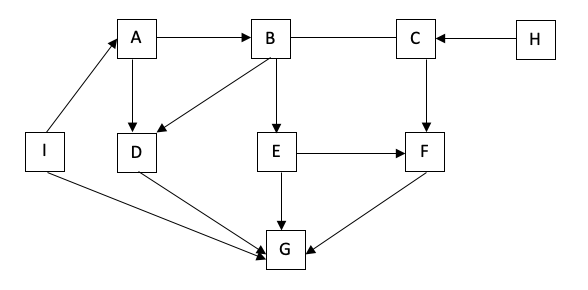
\includegraphics[scale=0.4]{dag1.png}
\end{figure}

\end{frame}

\begin{frame}{Causal diagram: Example}

\begin{figure}
	\centering 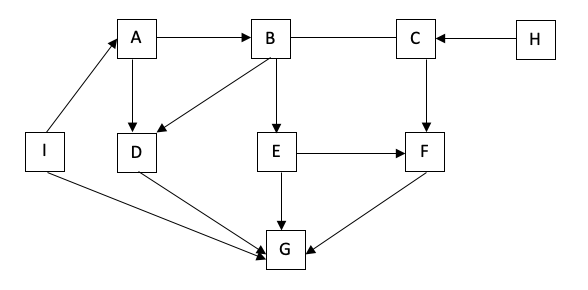
\includegraphics[scale=0.4]{dag1.png}
\end{figure}

\vspace{0.1cm} 

\textcolor{blue}{Question}: Which nodes (if any) are on a causal pathway from B to G? It may be useful to list the causal pathways first. \pause

\vspace{0.1cm}

\textcolor{blue}{Answer}: The causal pathways from B to G are: (B $\to$ D $\to$ G) (B $\to$ E $\to$ G) (B $\to$ E $\to$ F $\to$ G). Therefore, D, E, and F are on causal pathways from B to G.

\end{frame}

\subsection{Confounders}

% definition slide and example of diagram
\begin{frame}{Confounders}
Causal diagrams are useful tools we can use to determine whether or not variables are confounders.

\vspace{0.3cm}

\textcolor{blue}{Confounder} (or ``confounding variable"): a variable that is \textit{causally related to} our outcome, and also \textit{associated with} the exposure in our sample

\vspace{0.3cm} \pause

In a causal diagram, confounders look like \dots

\vspace{0.3cm}

\centering 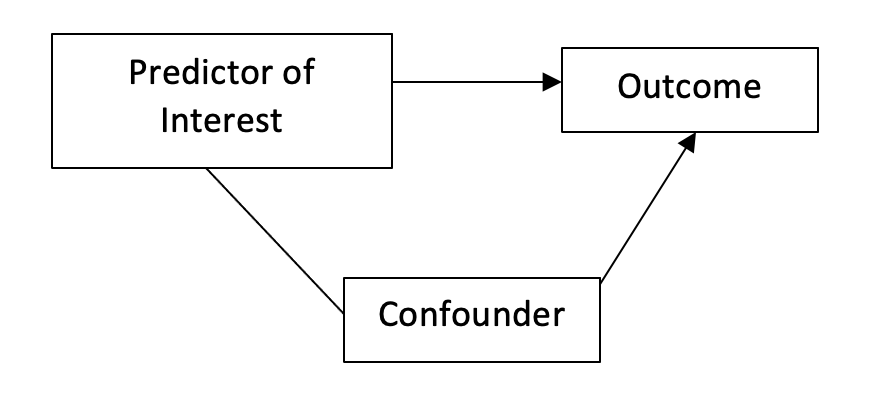
\includegraphics[scale=0.4]{confounder1.png}

\end{frame}

% second diagram example
\begin{frame}{Confounders}
Causal diagrams are useful tools we can use to determine whether or not variables are confounders.

\vspace{0.3cm}

\textcolor{blue}{Confounder} (or ``confounding variable"): a variable that is \textit{causally related to} our outcome, and also \textit{associated with} the exposure in our sample

\vspace{0.3cm} 

\dots confounders can also look like this\dots

\vspace{0.3cm}

\centering 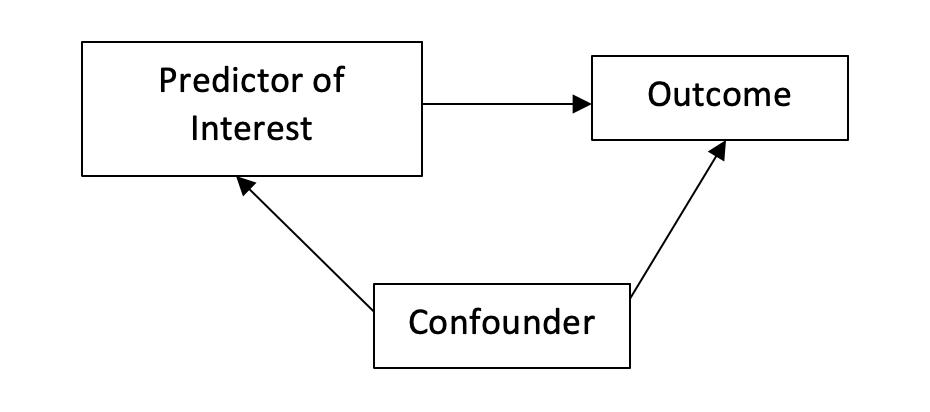
\includegraphics[scale=0.4]{confounder2.png}
\end{frame}

\begin{frame}{Confounders}
Causal diagrams are useful tools we can use to determine whether or not variables are confounders.

\vspace{0.3cm}

\textcolor{blue}{Confounder} (or ``confounding variable"): a variable that is \textit{causally related to} our outcome, and also \textit{associated with} the exposure in our sample

\vspace{0.3cm} 

\dots but confounders \textcolor{red}{cannot} look like this:

\vspace{0.3cm}

\begin{figure}
	\centering 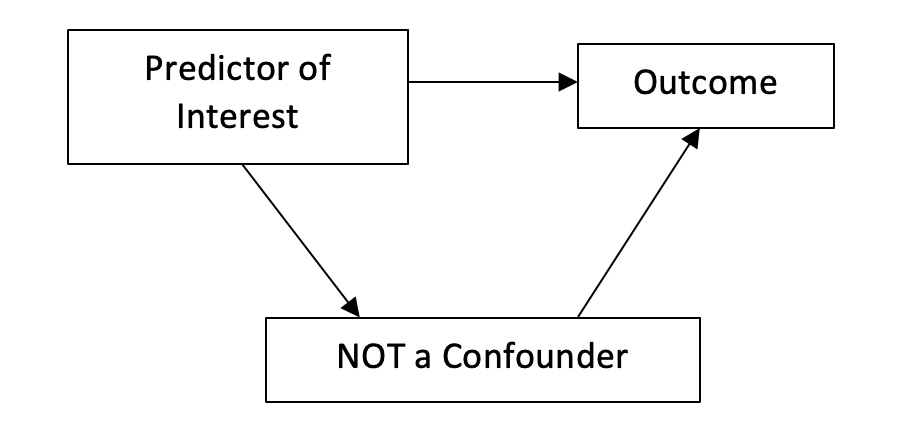
\includegraphics[scale=0.4]{confounder3.png}
\end{figure}


\small Confounder cannot be on the causal pathway from the predictor of interest to the outcome!

\end{frame}

% Example of what to look for graphically
\begin{frame}{Confounders: what to look for in a graph}
If your predictor of interest and outcome are both quantitative, and your potential confounder is \textit{binary}, there are some things you can look for in a graph that may indicate whether or not the potential confounder is in fact a confounding variable. \pause

\vspace{0.3cm}

Below we plot an exposure vs. an outcome:

\vspace{0.3cm}

\centering 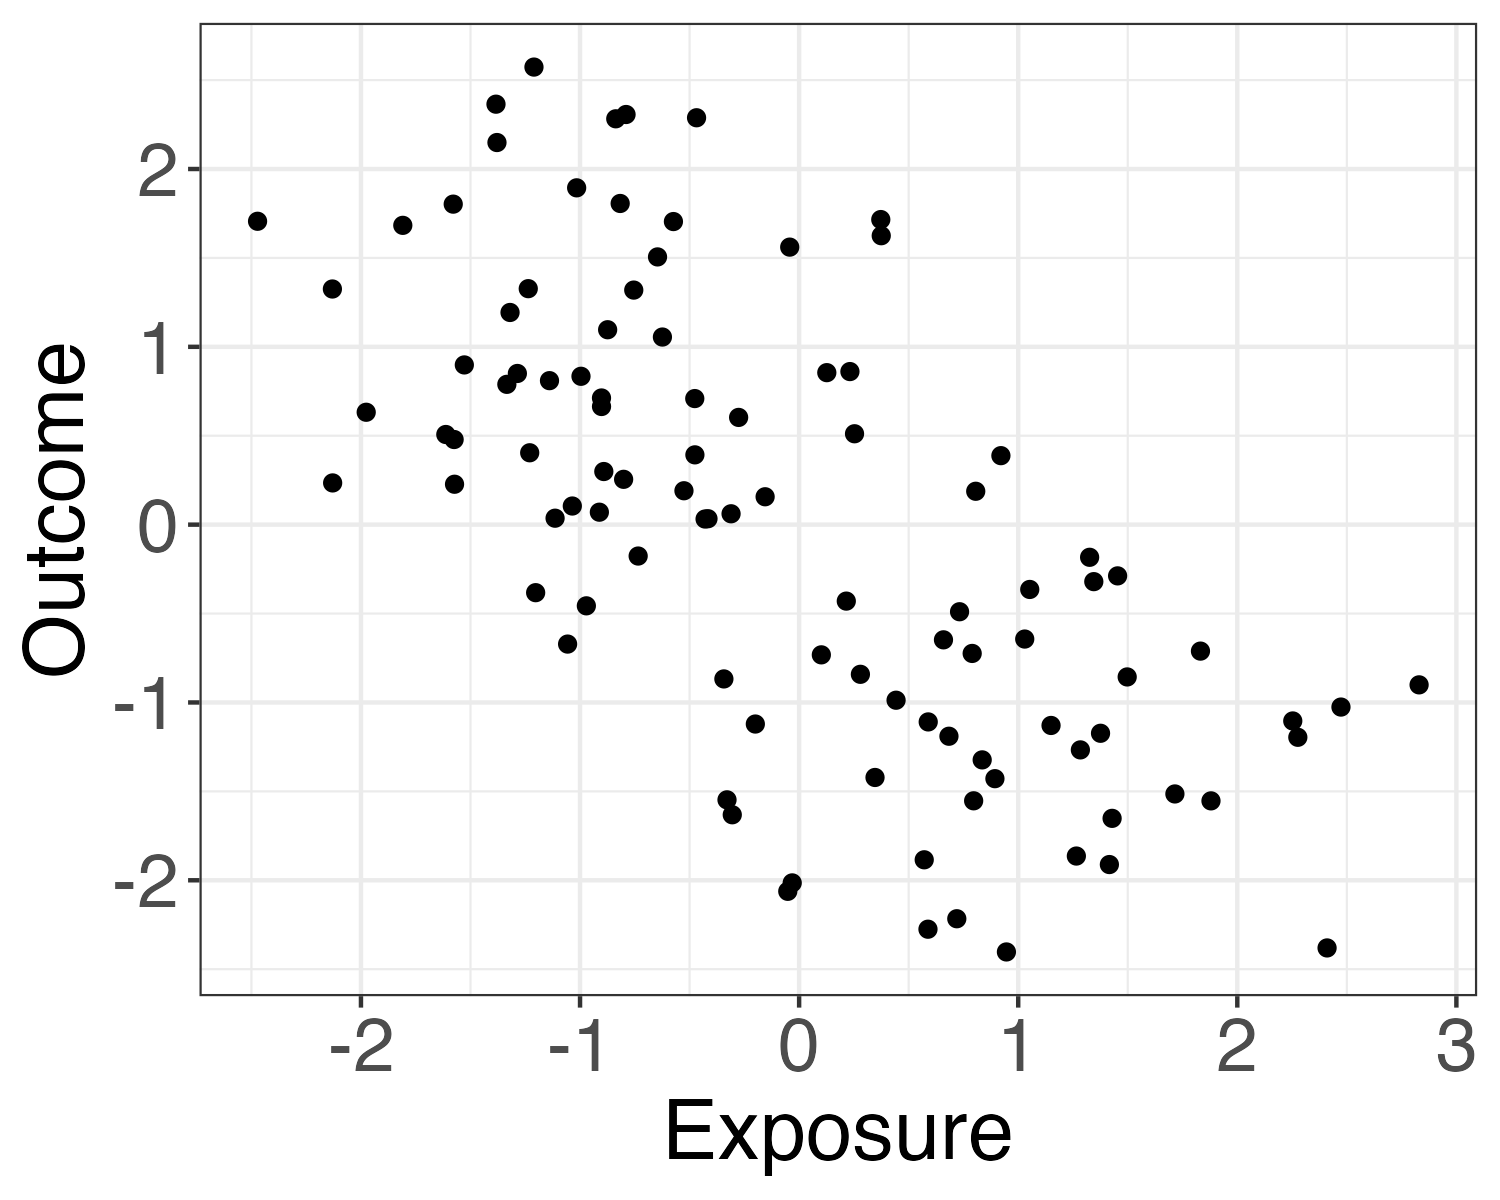
\includegraphics[scale=0.4]{p0.png}
\end{frame}

\begin{frame}{Confounders: what to look for in a graph}
We now color the points by our potential confounding variable.
\vspace{0.3cm}

\begin{figure}
	\centering 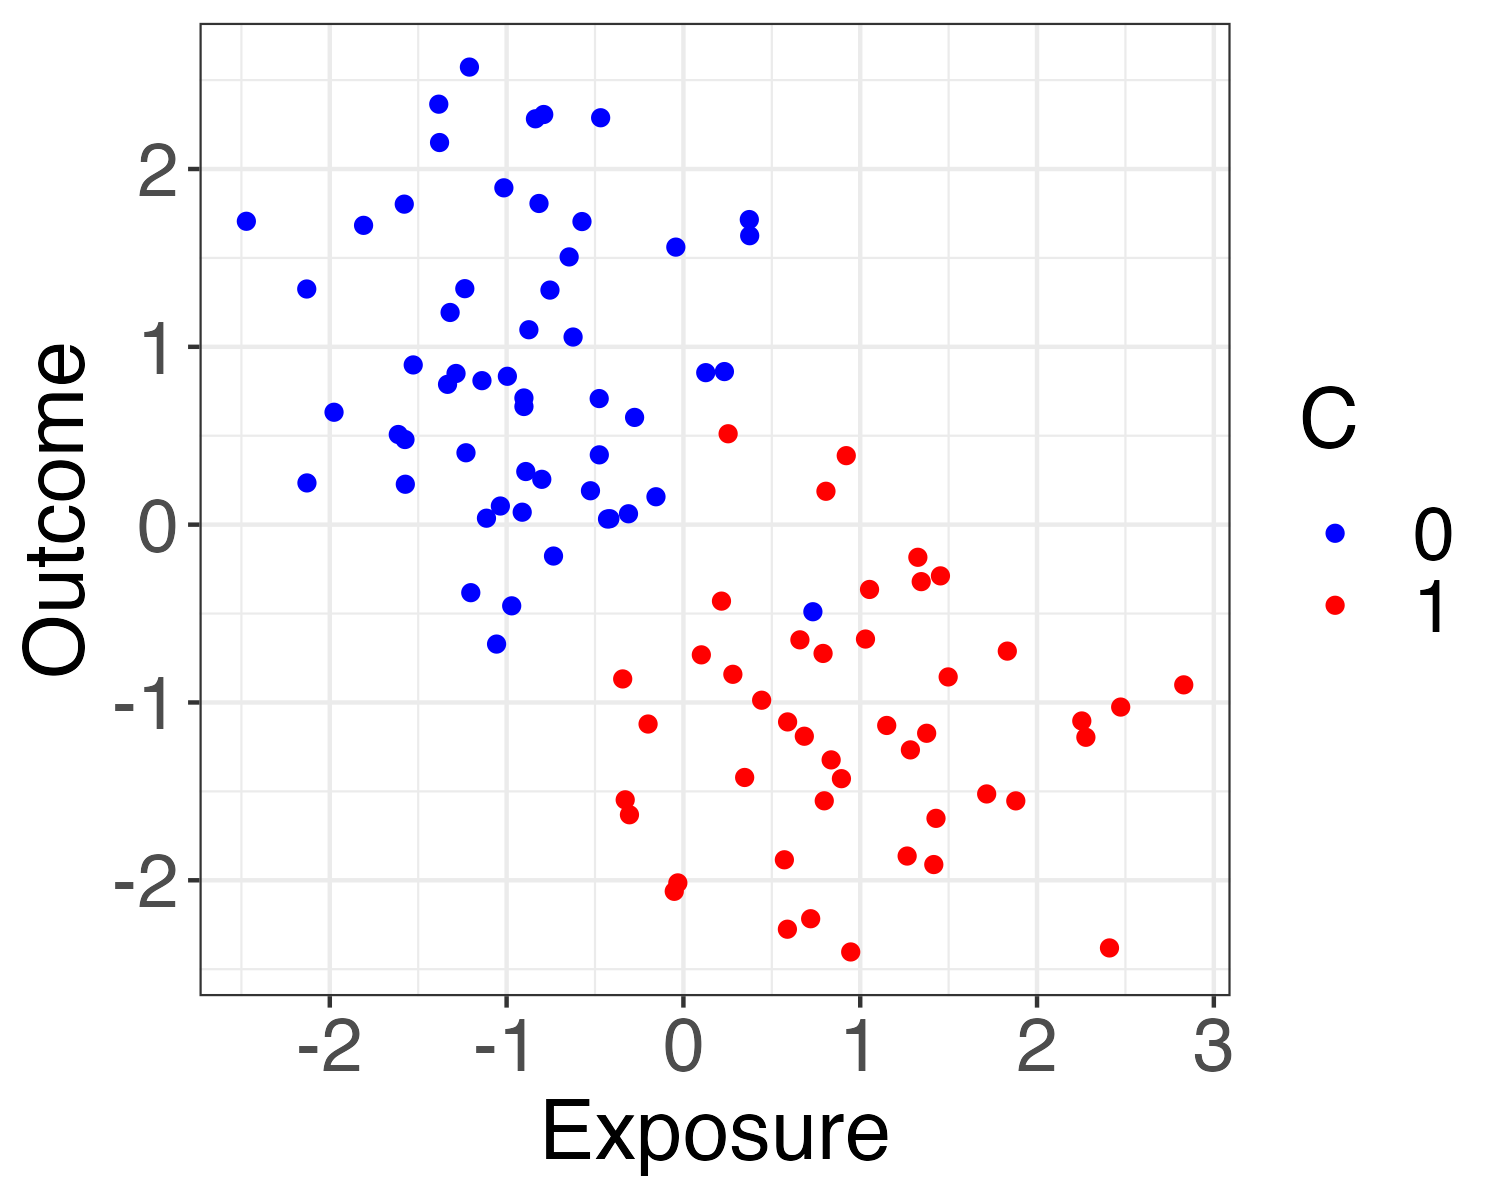
\includegraphics[scale=0.4]{p1.png}
\end{figure}

\vspace{0.3cm} \pause
\small We can see from the plot that the sets of points for each group identified by the potential confounder appear to be associated with the exposure (predictor of interest). This indicates that the potential confounder is associated with the predicted of interest \textit{in the sample} (one of the requirements for a confounding variable!).

\end{frame}

\begin{frame}{Confounders: what to look for in a graph}

\textcolor{red}{Important note}: A graph alone is not enough to determine if a variable is a confounder! You still need to think about whether that variable causes the outcome in the population, which cannot be determined graphically but must be thought about \textit{scientifically}.

\end{frame}

% Example with a question and answer - could be from the worksheet
\begin{frame}{Confounders: Example}

\textcolor{blue}{Question}: Your friend shows you the following graph\dots

\vspace{0.1cm}

\begin{figure}
	\centering 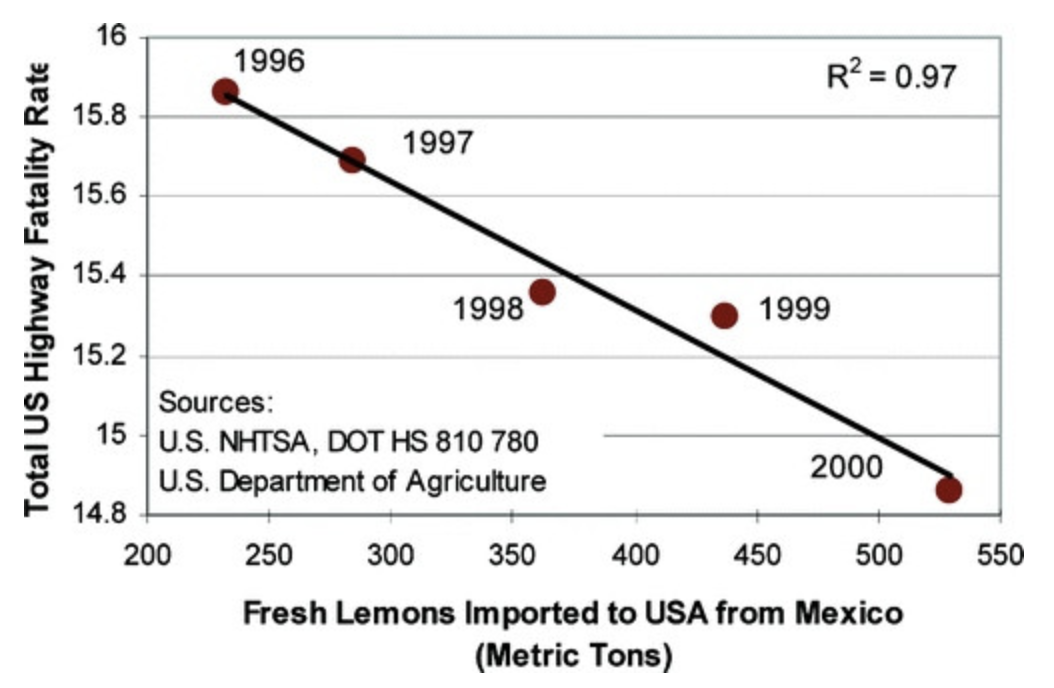
\includegraphics[scale=0.4]{lemons.png}
\end{figure}

\vspace{0.1cm} 

\dots and says ``More lemons imported from Mexico lead to lower highway fatality rates! We should import more lemons to lower the higher fatality rate!"



\end{frame}

\begin{frame}{Confounders: Example}
\begin{figure}
	\centering 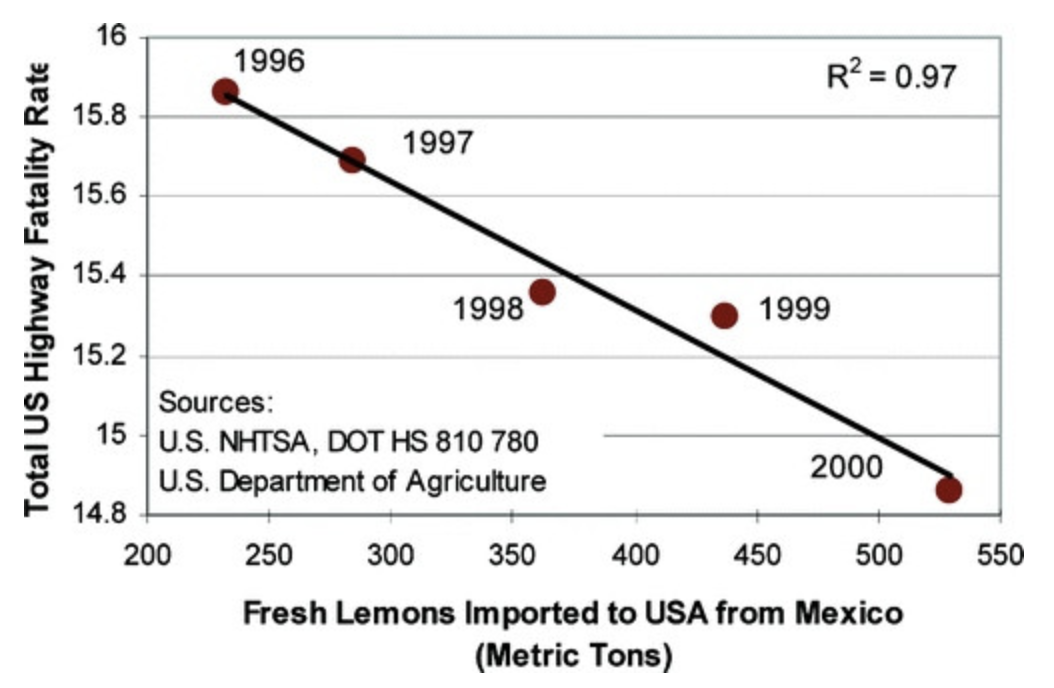
\includegraphics[scale=0.3]{lemons.png}
\end{figure}

\vspace{0.1cm} 

\dots and says ``More lemons imported from Mexico lead to lower highway fatality rates! We should import more lemons to lower the higher fatality rate!"

\vspace{0.3cm}

You think your friend is being mislead. What confounding variable is at play here, and what other possibly explanation could there be for this observed relationship?
\end{frame}

\begin{frame}{Confounders: Example}
\textcolor{blue}{Question}: You think your friend is being mislead. What confounding variable is at play here, and what other possibly explanation could there be for this observed relationship?

\vspace{0.3cm}

\textcolor{blue}{Answer}: From the graph, we can see that highway fatality rates have decreased over time, and number of lemons imported has increased \textit{over time}. Time is a confounding variable in this case. Highway fatality rates have likely decreased over time because cars have gotten much safer with improved airbag quality and other innovations. Number of fresh lemon imported has increased over time, potentially because the US population has increased (and therefore demands more lemons).
\end{frame}


\begin{frame}{Confounders and study design}
When our scientific question involves a causal relationship, whether or not we \textit{need} to adjust for covariates depends on the study design.

\vspace{0.3cm}

When reviewing study design, we said that a randomized controlled trial is the only study design in which we can confidently make causal claims about relationships between variables. \textit{However}, if we are able to adjust for \textit{all possible confounders} in an observational study, we could also make causal statements for these study designs. In practice, situations where we can confidently say we've adjusted for all possible confounders are extremely rare. Nevertheless, it is good to adjust for any possible confounders we have regardless, so long as we are still answering a scientific question of interest. \pause

\vspace{0.3cm}

\begin{itemize}
	\item \textcolor{blue}{Randomized controlled trial:} no need to adjust because there are no possible confounders (unless randomization has failed)
	\item \textcolor{blue}{Observational study:} must adjust for all possible confounders in order to make causal claims, should adjust for all potential confounders regardless
\end{itemize}
\end{frame}

\begin{frame}{Confounders: regression equation}
Writing regression equations including confounding variables is as simple as adding in an additional covariate. Suppose

\vspace{0.3cm}

\begin{itemize}
	\item $Y$ = outcome
	\item $X$ = predictor of interest
	\item $Z$ = confounder
\end{itemize}

\vspace{0.3cm}

Then to include the confounding variable $Z$ into our model, we would write
$$
E[Y \mid X, Z] = \beta_0 + \beta_1 X + \beta_2 Z
$$

If we instead had \textit{two} confounding variables $Z$ and $W$, we would write
$$
E[Y \mid X, Z, W] = \beta_0 + \beta_1 X + \beta_2 Z + \beta_3 W
$$
\dots and so forth with additional confounding variables!

\end{frame}

\subsection{Effect modifiers}

% definition slide and example of diagram
\begin{frame}{Effect modifiers}
Causal diagrams are \textit{also} useful tools we can use to determine whether or not variables are effect modifiers.

\vspace{0.3cm}

\textcolor{blue}{Effect modifiers}: a variable that modifies the association between the predictor of interest and the outcome. In other words, the association between the predictor of interest and the outcome \textit{depends on} the effect modifier \pause

\vspace{0.3cm}

In a causal diagram, we denote effect modifiers like this:

\vspace{0.1cm}

\begin{figure}
	\centering 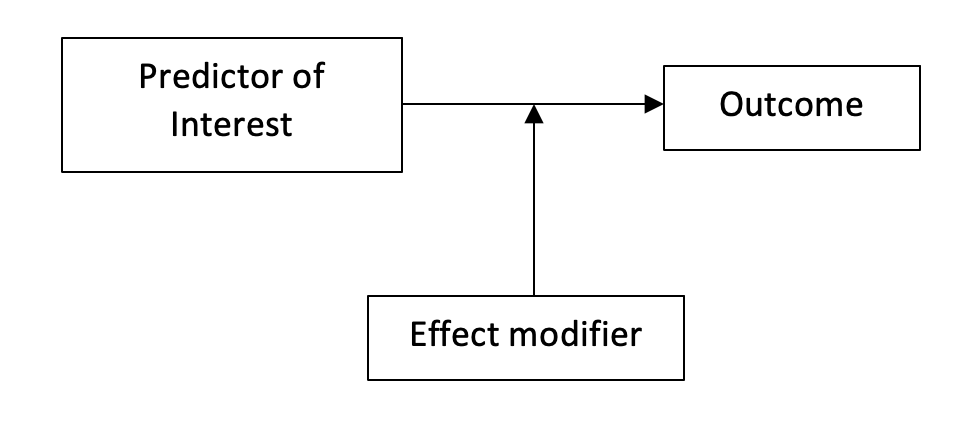
\includegraphics[scale=0.4]{effectmod1.png}
\end{figure}
\end{frame}


% Example of what to look for graphically
\begin{frame}{Effect modifiers: what to look for in a graph}
If your predictor of interest and outcome are both quantitative, and your potential effect modifier is \textit{binary}, there are some things you can look for in a graph that may indicate whether or not the potential effect modifier is in fact an effect modifier. \pause

\vspace{0.3cm}

Below we plot an exposure vs. an outcome:

\vspace{0.3cm}

\centering 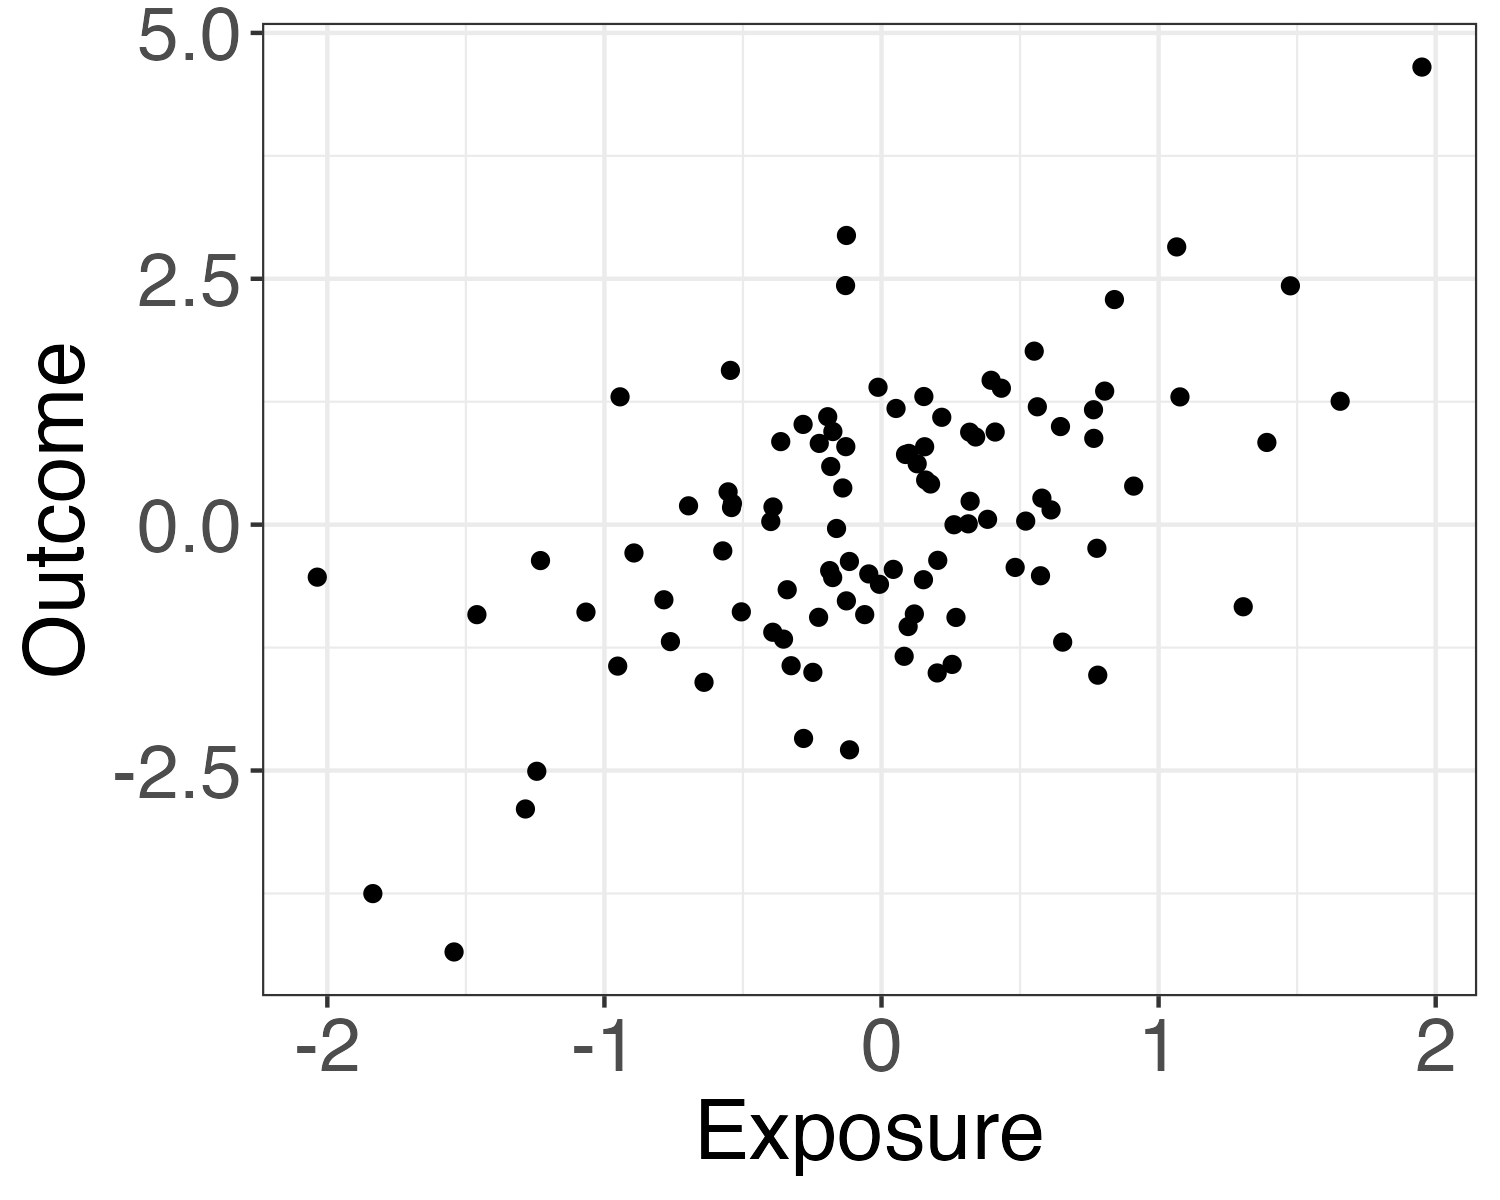
\includegraphics[scale=0.4]{p2.png}
\end{frame}

\begin{frame}{Effect modifiers: what to look for in a graph}
We now color the points by our potential effect modifier\dots
\vspace{0.3cm}

\begin{figure}
	\centering 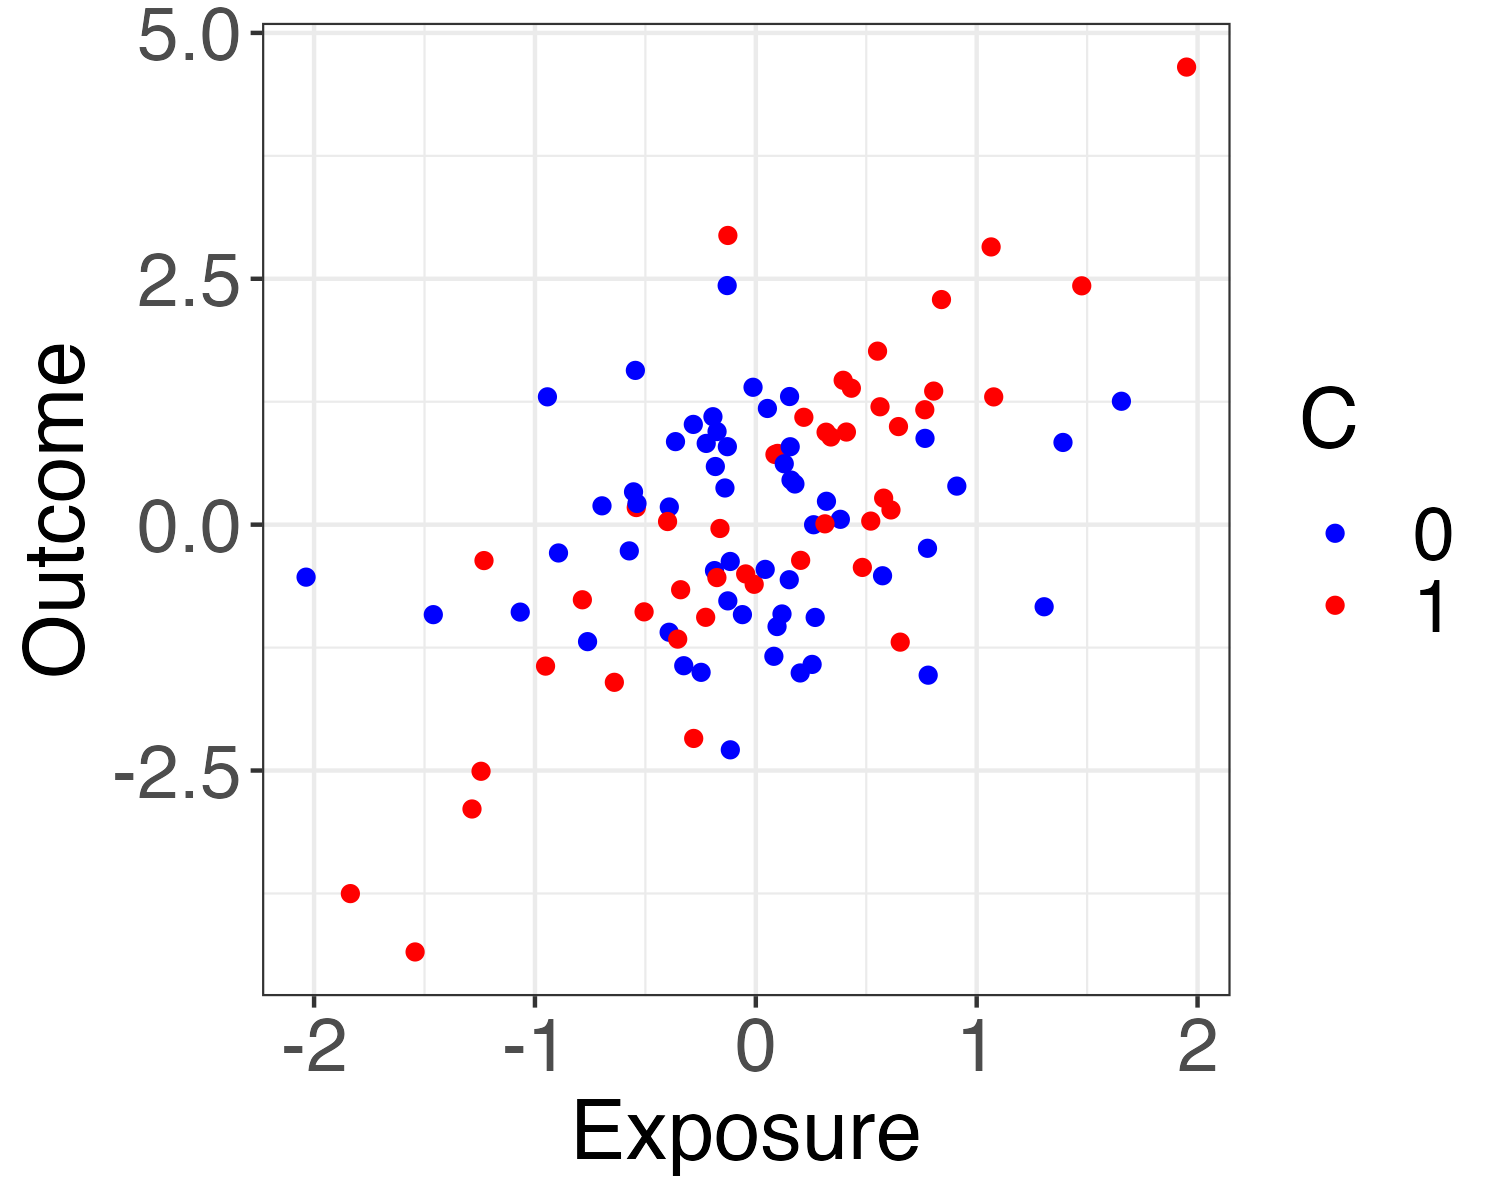
\includegraphics[scale=0.4]{p3.png}
\end{figure}

\end{frame}

\begin{frame}{Effect modifiers: what to look for in a graph}
\dots and if we were to fit simple linear regressions for each group defined by our potential effect modifier (a stratified analysis), we could add those regression lines to the plot as well:

\vspace{0.3cm}

\begin{figure}
	\centering 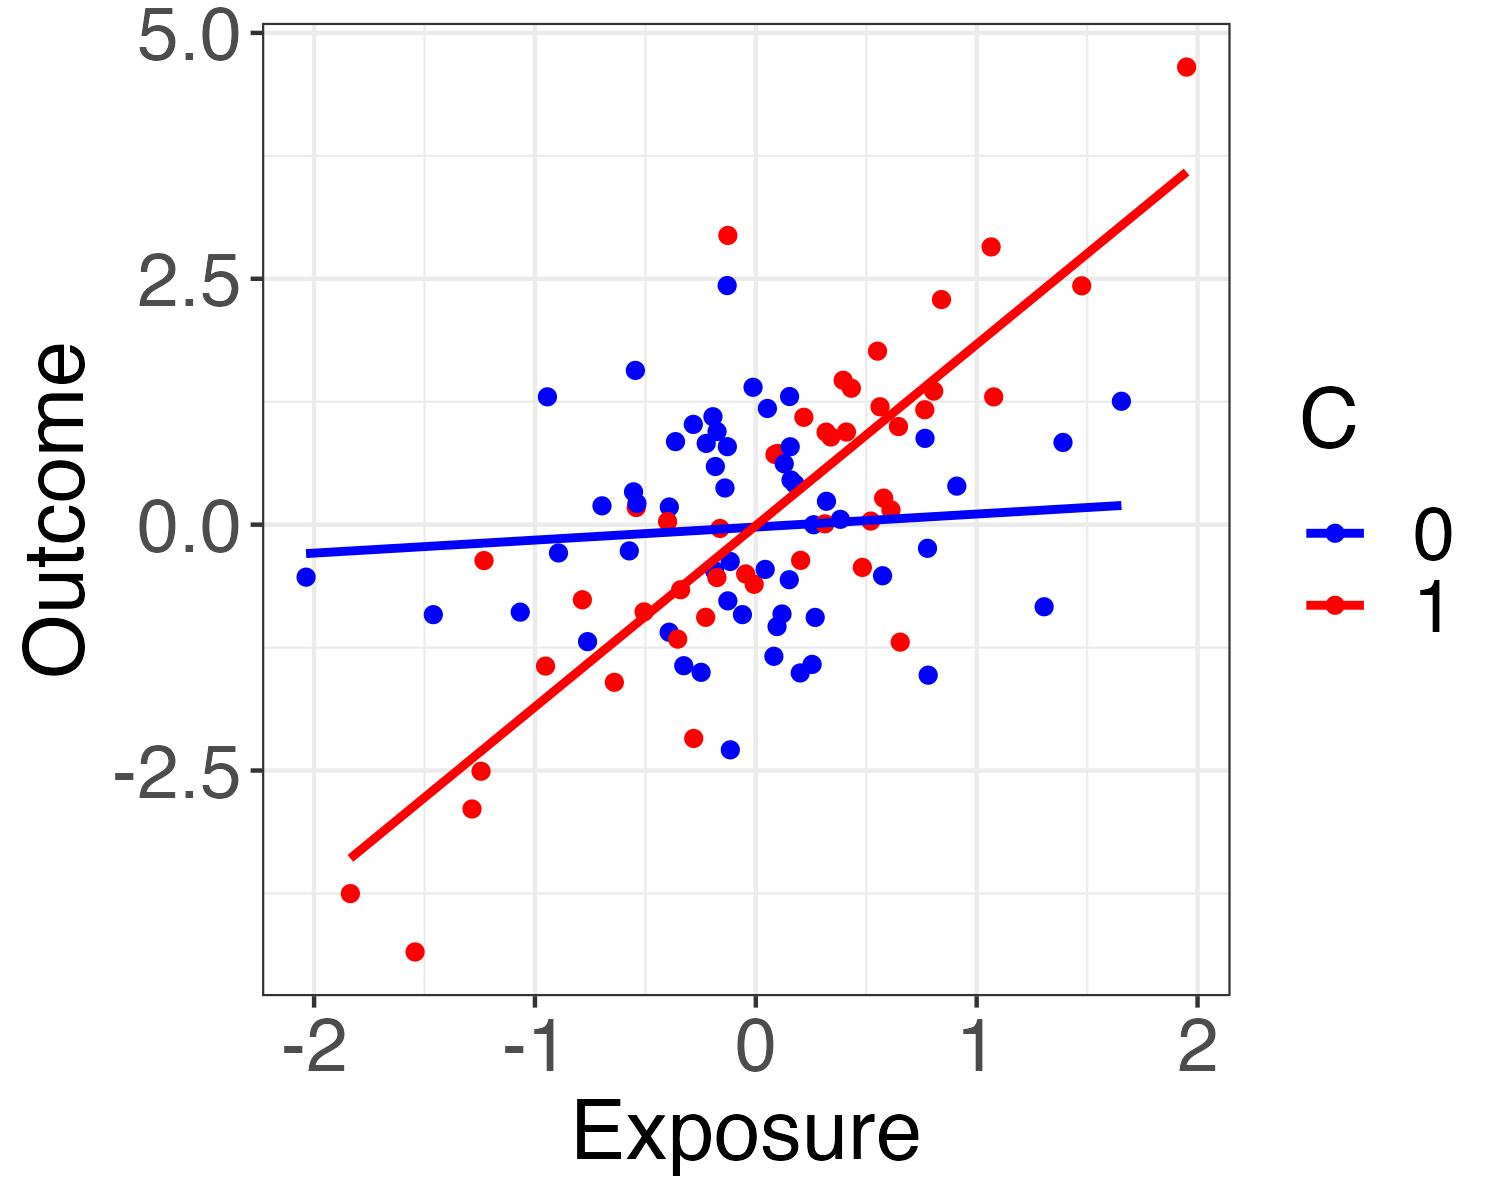
\includegraphics[scale=0.4]{p4.png}
\end{figure}

\end{frame}

\begin{frame}{Effect modifiers: what to look for in a graph}

\begin{figure}
	\centering 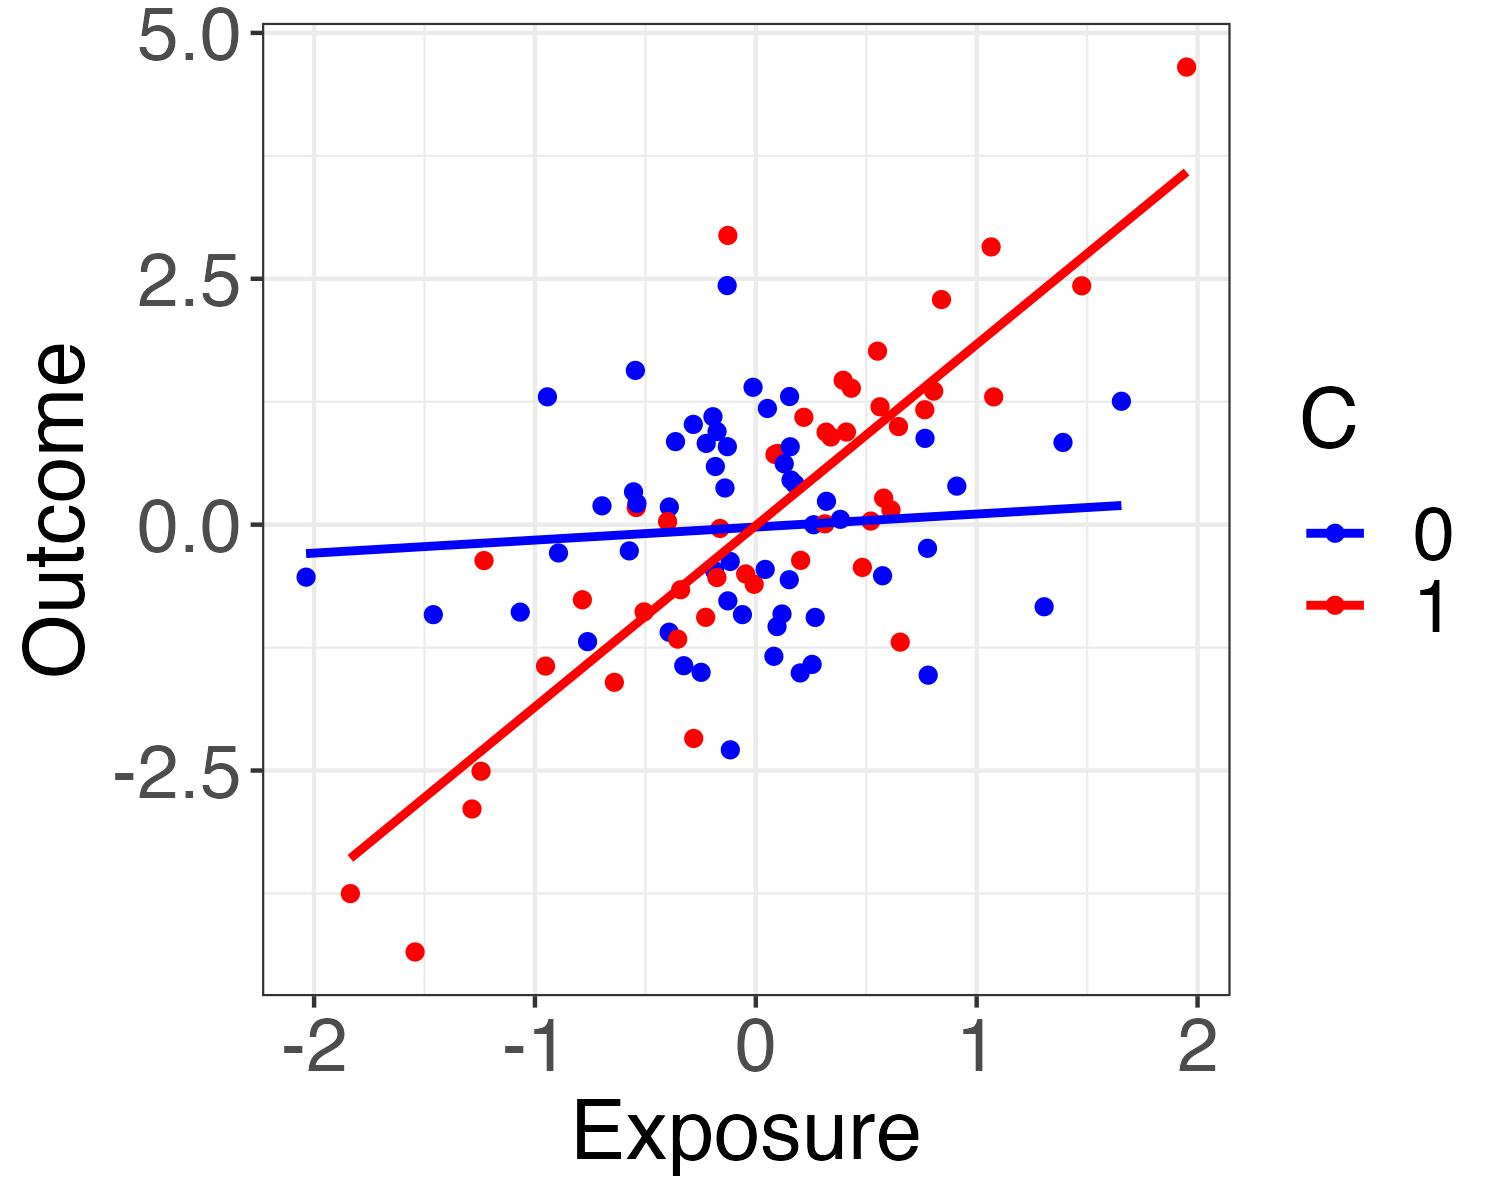
\includegraphics[scale=0.4]{p4.png}
\end{figure}

\vspace{0.3cm}

The key thing to note here is that groups defined by a binary effect modifier will have linear regression lines with different \textcolor{blue}{slopes} \textit{and} different \textcolor{blue}{intercepts}. This indicates that the association between the exposure and the outcome has been \textit{modified} by the additional variable, and thus the additional variable is an effect modifier.

\end{frame}

\begin{frame}{Effect modifiers: always adjust}
When our scientific question addresses whether or not the assication between a predictor of interest and the outcome differs by an additional covariate (effect modifier), you \textit{must} adjust for the covariate in your model. Otherwise, your model would not adequately answer the scientific question.

\vspace{0.3cm}

(Note that this is different from a confounder, where we do not need to adjust for confounding variables in a randomized controlled trial, so long as randomization was successful.)


\end{frame}

\begin{frame}{Effect modifiers: regression equation}
The presence of an effect modifier is called an \textcolor{blue}{interaction}, and means we will need to include an interaction \textit{term} in our statistical model. In regression equations, interaction terms are modeled as the \textit{multplication} of the potential effect modifier and the predictor of interest. Suppose
\vspace{0.3cm}

\begin{itemize}
	\item $Y$ = outcome
	\item $X$ = predictor of interest
	\item $Z$ = potential effect modifier
\end{itemize}

\vspace{0.3cm}

Then to include the potential effect modifier into our model, we would write,
$$
E[Y \mid X, Z] = \beta_0 + \beta_1 X + \beta_2 Z + \beta_3 (X \times Z)
$$
\end{frame}

\begin{frame}{Effect modifiers: regression equation}
$$
E[Y \mid X, Z] = \beta_0 + \beta_1 X + \beta_2 Z + \beta_3 (X \times Z)
$$
New terminology:

\vspace{0.3cm}

\begin{itemize}
	\item The terms $X$ and $Y$ are called \textcolor{blue}{main effects}
	\item The multiplicative term $(X \times Z)$ is called the \textcolor{blue}{interaction term}
\end{itemize}

\vspace{0.3cm}

You must \textcolor{red}{always} include the main effects in your model if you include an interaction term. Not including the main effects changes the interpretation of the interaction term. We'll give examples of interpretation in a bit.

\end{frame}

\subsection{Precision variables}

% definition slide and example of diagram
\begin{frame}{Precision variables}
Causal diagrams can also help us determine whether or not variables are precision variables.

\vspace{0.3cm}

\textcolor{blue}{Precision variable}: a variable that is associated with (or causes) the outcome \textit{in the population}, but is not associated with the predictor of interest \textit{in the sample} \pause

\vspace{0.3cm}

In a causal diagram, we denote precision variables as\dots

\vspace{0.3cm}

\centering 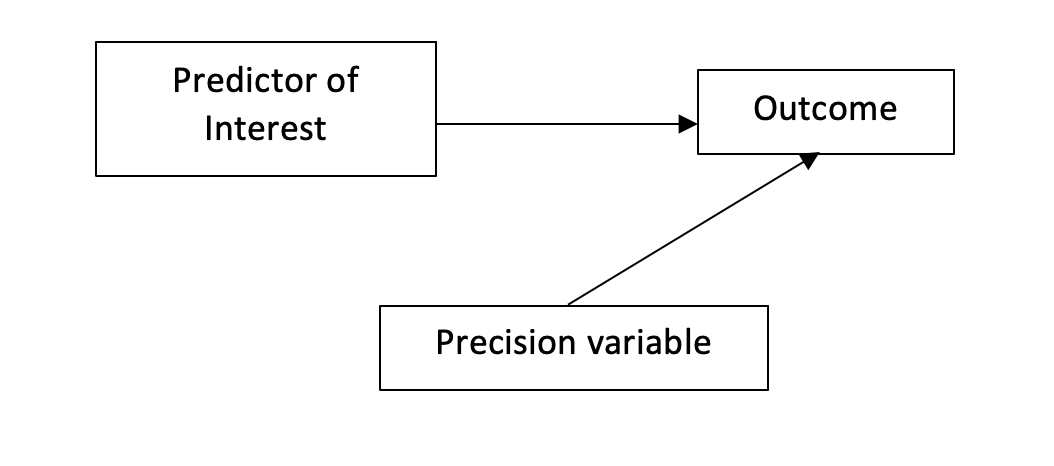
\includegraphics[scale=0.4]{precvar1.png}

\end{frame}

\begin{frame}{Precision variables}
Causal diagrams can also help us determine whether or not variables are precision variables.

\vspace{0.3cm}

\textcolor{blue}{Precision variable}: a variable that is associated with (or causes) the outcome \textit{in the population}, but is not associated with the predictor of interest \textit{in the sample} 

\vspace{0.3cm}

\dots or we denote precision variables as:

\vspace{0.3cm}

\centering 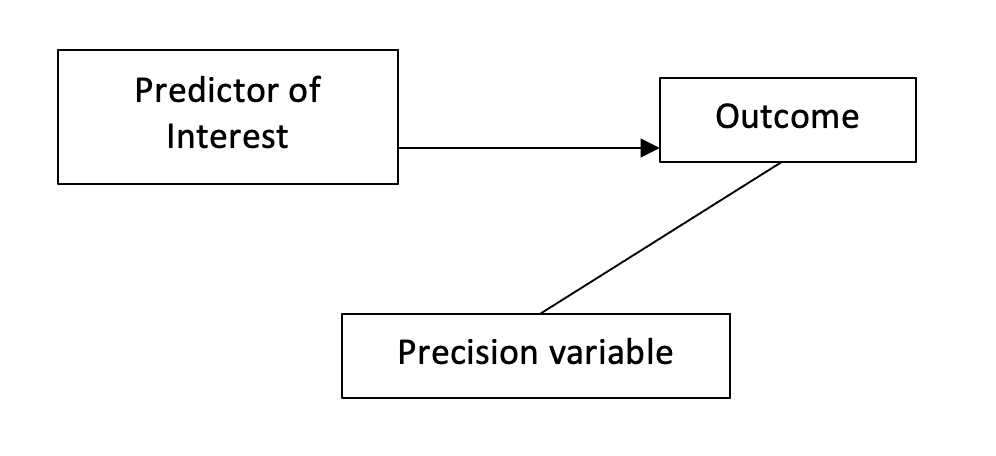
\includegraphics[scale=0.4]{precvar2.png}
\end{frame}

% Example of what to look for graphically in R
\begin{frame}{Precision variable: what to look for in a graph}
If your predictor of interest and outcome are both quantitative, and your potential precision variable is \textit{binary}, there are some things you can look for in a graph that may indicate whether or not the potential precision variable is in fact a precision variable. \pause

\vspace{0.3cm}

Below we plot an exposure vs. an outcome:

\vspace{0.1cm}

\centering 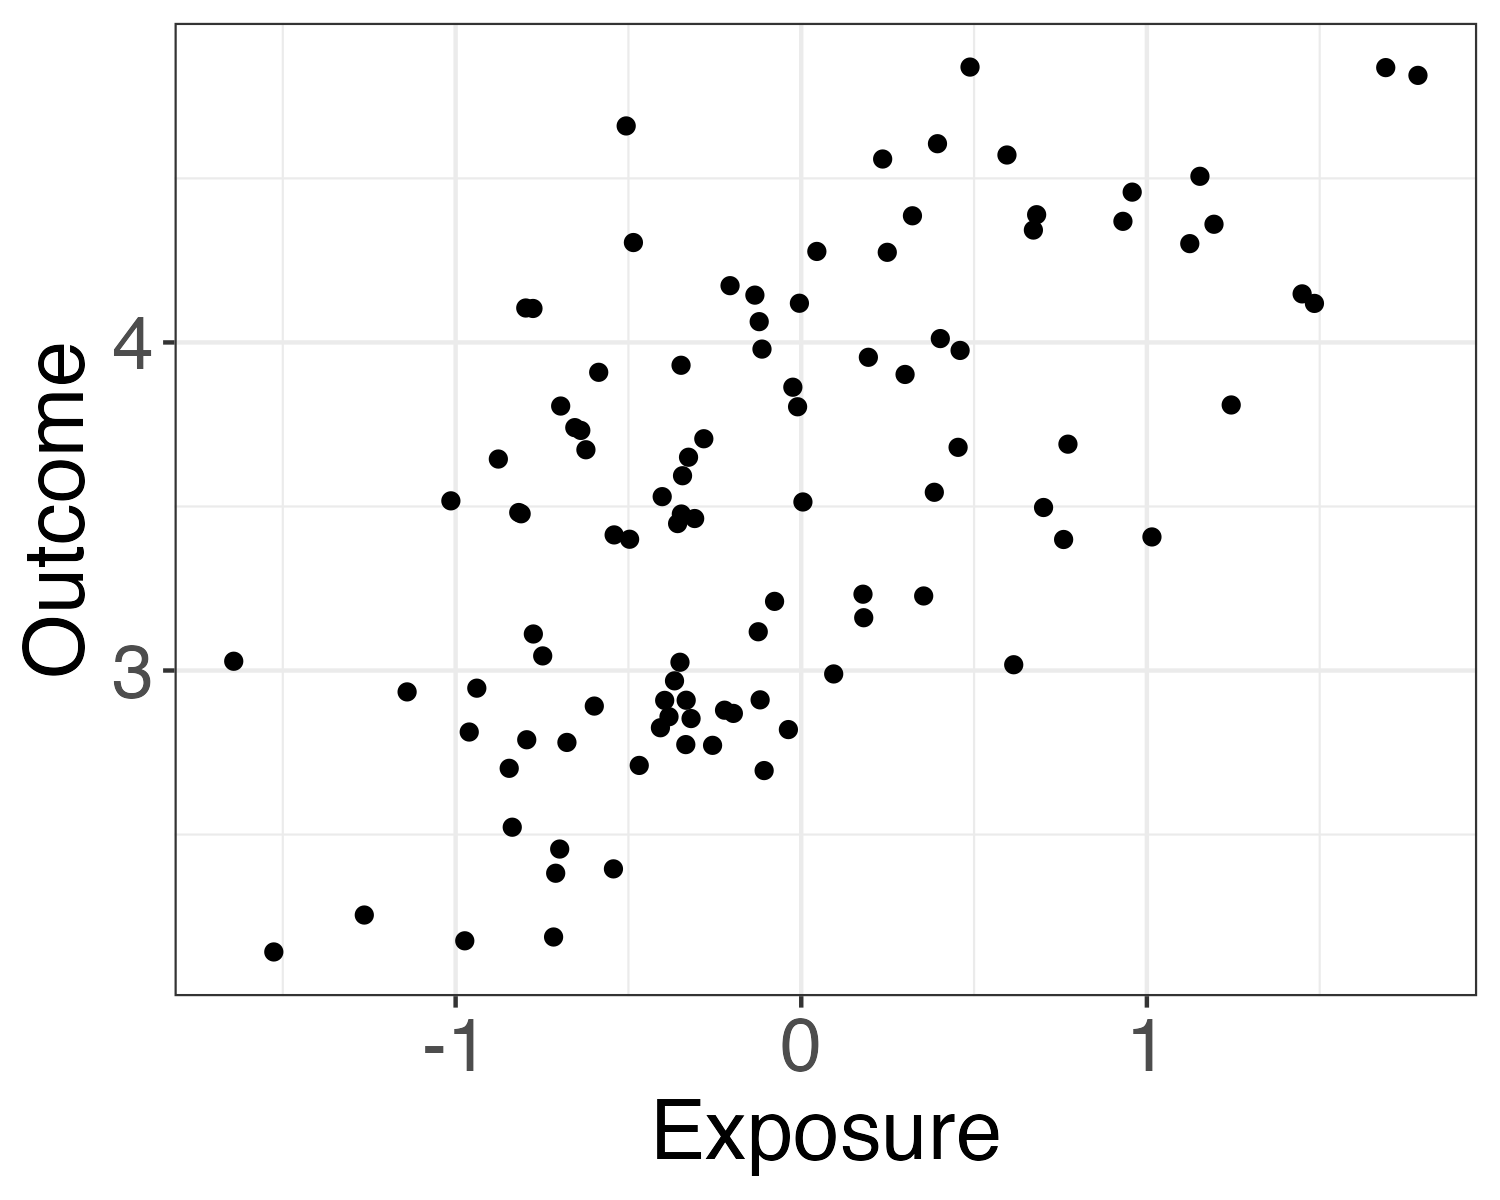
\includegraphics[scale=0.4]{p5.png}
\end{frame}

\begin{frame}{Precision variables: what to look for in a graph}
We now color the points by our potential precision variable\dots

\vspace{0.3cm}

\centering 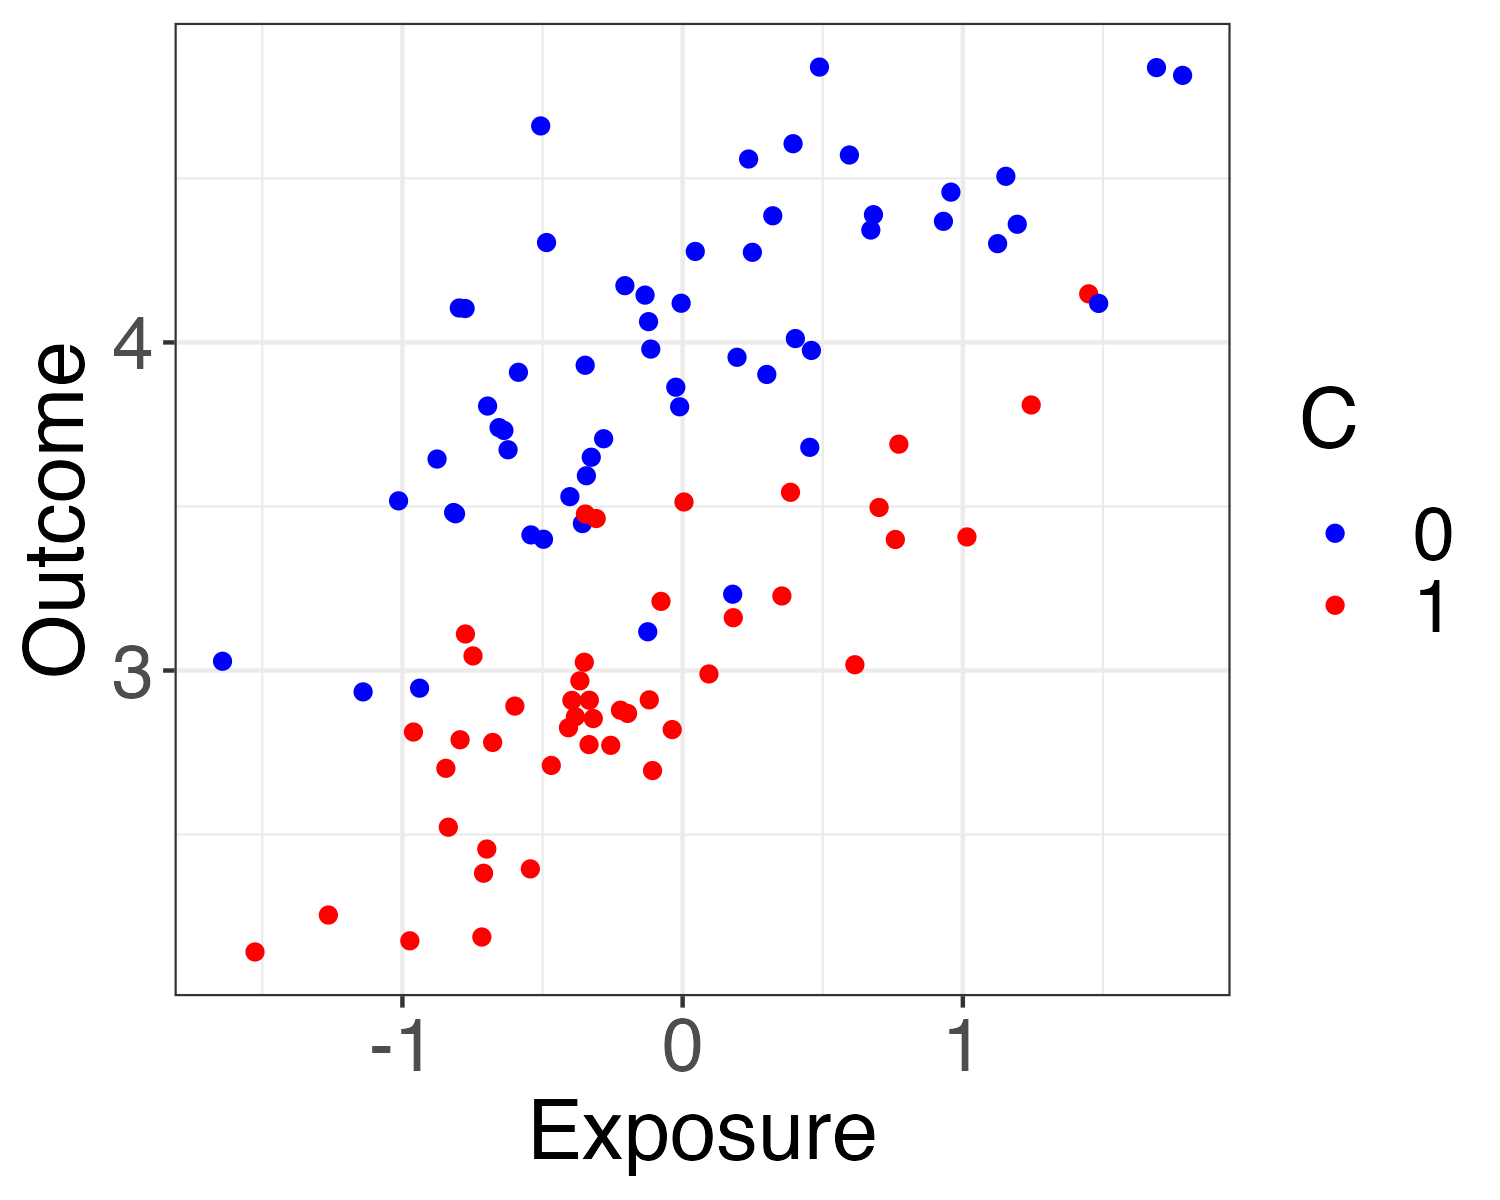
\includegraphics[scale=0.4]{p6.png}

\end{frame}

\begin{frame}{Precision variables: what to look for in a graph}
\dots and if we were to fit simple linear regressions for each group defined by our potential precision variable (a stratified analysis), we could add those regression lines to the plot as well:

\vspace{0.3cm}

\centering 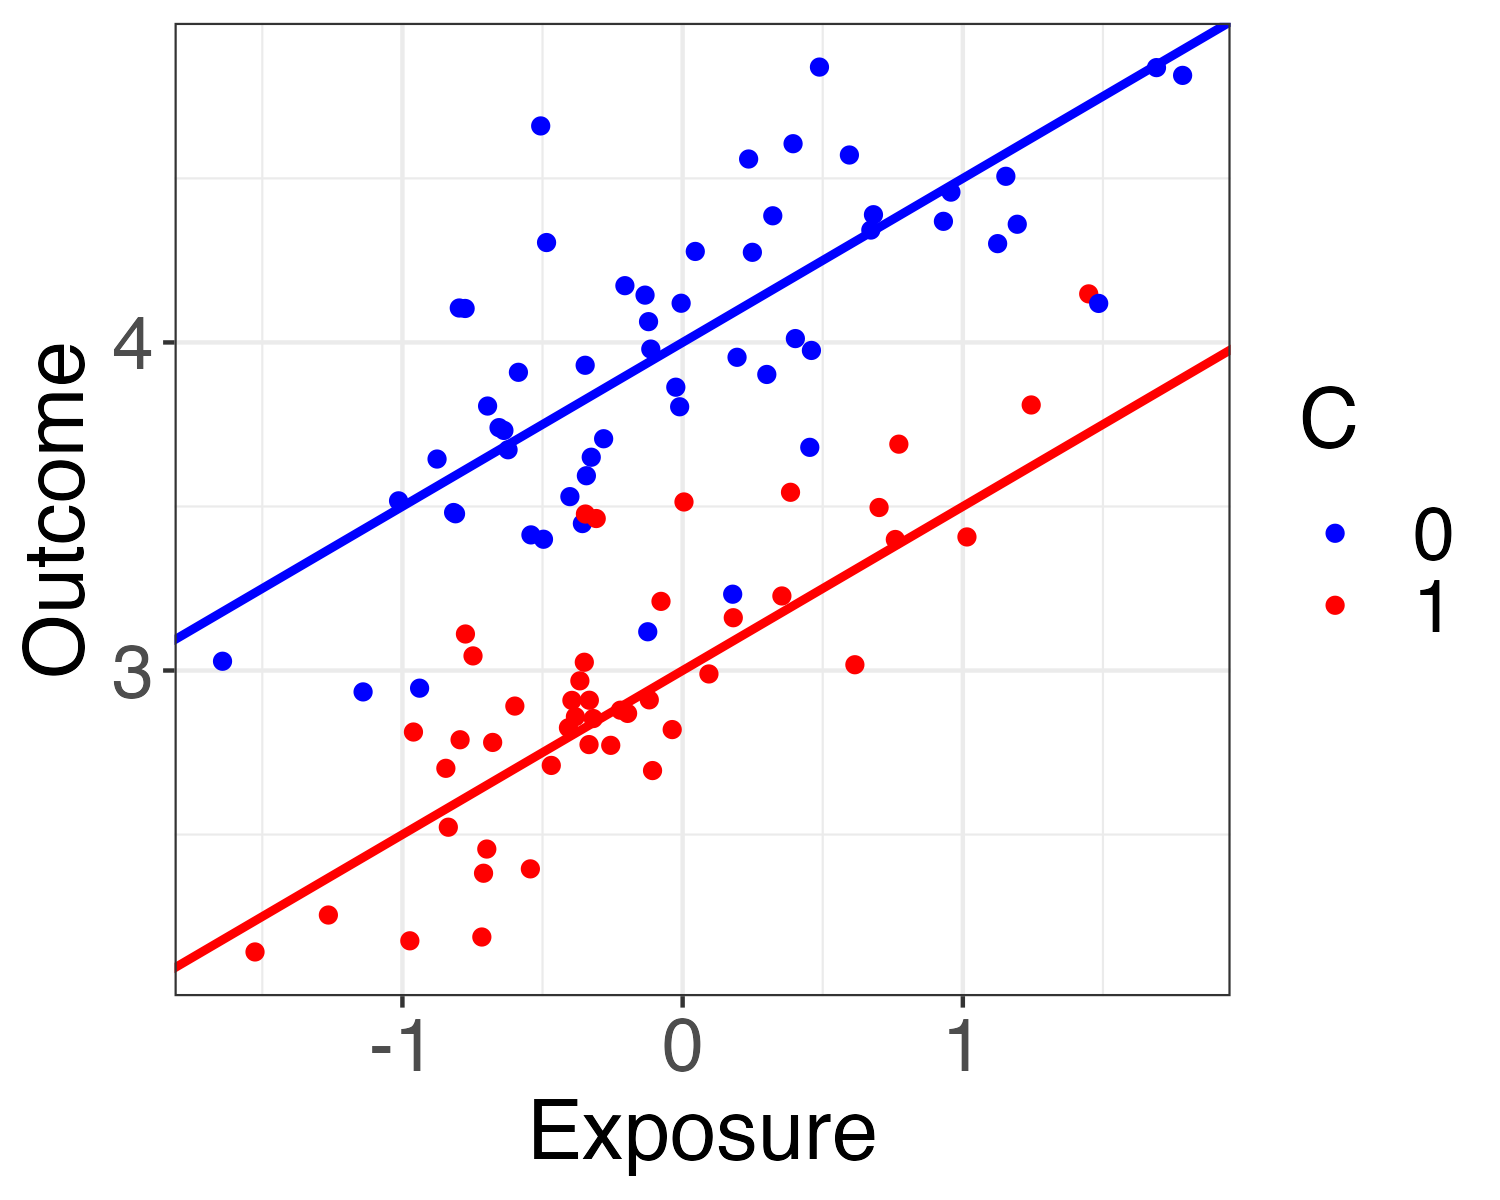
\includegraphics[scale=0.4]{p7.png}

\end{frame}

\begin{frame}{Precision variables: what to look for in a graph}
\begin{figure}
	\centering 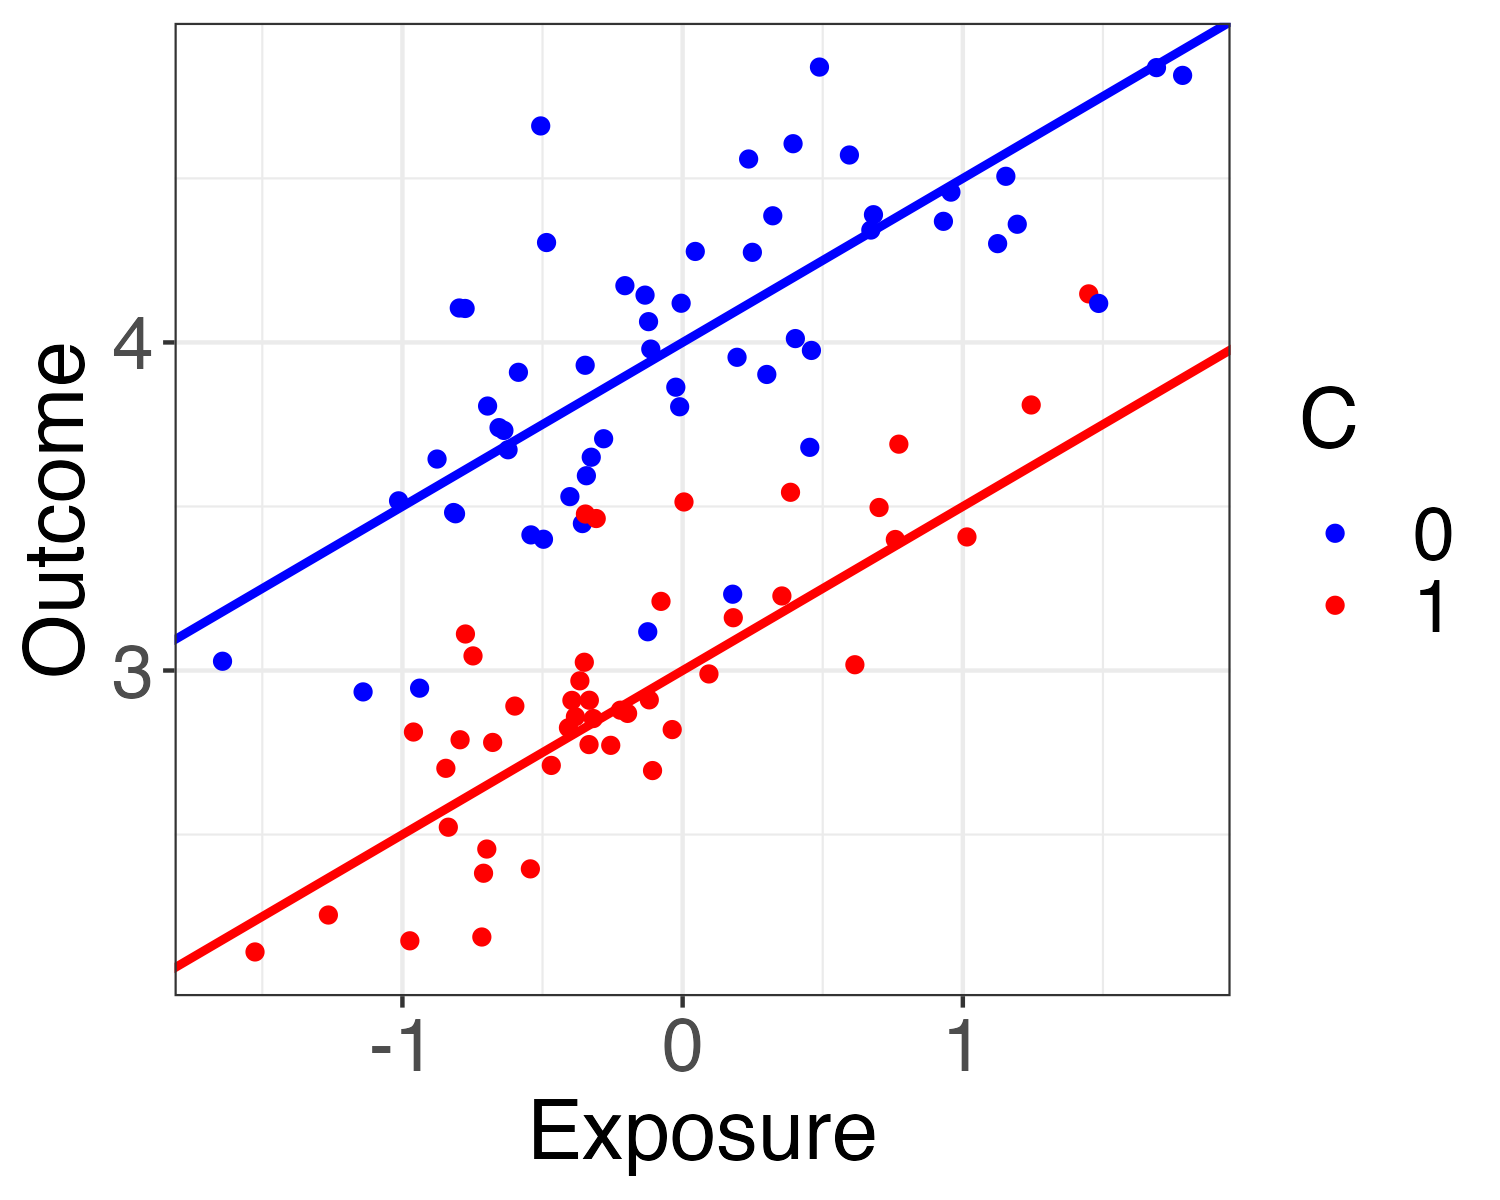
\includegraphics[scale=0.4]{p7.png}
\end{figure}

\vspace{0.3cm}

The key thing to note here is that the groups defined by a binary precision variable will have linear regression lines with different \textcolor{blue}{intercepts}, but the \textit{same} \textcolor{blue}{slope}. This indicates that there is no association between the exposure and additional variable, and hints that there may be a relationship between the additional variable and the outcome in the population. 
\end{frame}

\begin{frame}{Precision variables: what to look for in a graph}
\textcolor{red}{Important note}: A graph alone is not enough to determine if a variable is a precision variable! You still need to think about whether that variable is associated with the outcome \textit{in the population}. This should generally be true if your data is representative of your population.
\end{frame}

\begin{frame}{Precision variables: regression equation}
Writing regression equations including precision variables is as simple as adding in an additional covariate (just like with confounders). Suppose

\vspace{0.3cm}

\begin{itemize}
	\item $Y$ = outcome
	\item $X$ = predictor of interest
	\item $Z$ = precision variable
\end{itemize}

\vspace{0.3cm}

Then to include the precision variable $Z$ into our model, we would write
$$
E[Y \mid X, Z] = \beta_0 + \beta_1 X + \beta_2 Z
$$

If we instead had \textit{two} precision variables $Z$ and $W$, we would write
$$
E[Y \mid X, Z, W] = \beta_0 + \beta_1 X + \beta_2 Z + \beta_3 W
$$
\dots and so forth with additional precision variables!

\end{frame}


% Example with a question and answer - could be from the worksheet

\subsection{Stratification}

% maybe move this entire subsection up to the beginning of Adjusting for covariates? or make it it's own section beforehand?



% motivator for multiple linear regression
% note that also had multiple coefficients with the polynomial transformation


\begin{frame}[c]
\centering \huge Any Questions?
\end{frame}

\end{document}